\documentclass[12pt]{article}
\usepackage{geometry}
\geometry{left=1in,right=0.75in,top=1in,bottom=1in}

\newcommand{\Problem}{B}
\newcommand{\Team}{2418525}


\usepackage[english]{babel}
\usepackage{newtxtext}
\usepackage{amsmath,amssymb,amsthm}
\usepackage{newtxmath} % must come after amsXXX
\usepackage{booktabs}
\usepackage{multicol}
\usepackage{graphicx}
\usepackage{xcolor}
\usepackage{fancyhdr}
\usepackage{hyperref}
\usepackage{subfigure}
\usepackage{tikz}
\usepackage{tikz-3dplot}
\usepackage{multirow}
\usepackage{wallpaper}
\usepackage[numbers]{natbib}

\usetikzlibrary{3d}

% no color
\hypersetup{
    colorlinks=false,
    pdfborder={0 0 0},
}

\lhead{Team \Team}
\rhead{}
\cfoot{}
\newtheorem{theorem}{Theorem}
\newtheorem{corollary}[theorem]{Corollary}
\newtheorem{lemma}[theorem]{Lemma}
\newtheorem{definition}{Definition}


\begin{document}
\DeclareGraphicsExtensions{.pdf, .jpg, .tif, .png}
\thispagestyle{empty}
\vspace*{-16ex}
\centerline{
    \begin{tabular}{*3{c}}
        \parbox[t]{0.3\linewidth}{\begin{center}\textbf{Problem Chosen}\\ \Large \textcolor{red}{\Problem}\end{center}}
         & \parbox[t]{0.3\linewidth}{\begin{center}\textbf{2024\\ MCM/ICM\\ Summary Sheet}\end{center}}
         & \parbox[t]{0.3\linewidth}{\begin{center}\textbf{Team Control Number}\\ \Large \textcolor{red}{\Team}\end{center}} \\
        \hline
    \end{tabular}
}

% Set the default font to Times New Roman
% \renewcommand{\rmdefault}{ptm}
% \renewcommand{\sfdefault}{phv}
% set the default font size to 12pt

\begin{center}
    \LARGE \textbf{Journey to the Rescue: \\Submersibles in the Deep Sea}
\end{center}

% \vspace{.5cm}

\begin{center}
    \large \textbf{Summary}
\end{center}


There has always been great interest in the exploration of the oceans, and submersibles have been developed to investigate these vast and enigmatic regions. However, there are inherent risks associated with submersible exploration, especially in unknown and deep ocean environments. As the depth of exploration increases, so does the likelihood of submersible malfunctions. Thus, this paper aims to enhance the search and rescue capabilities for lost submersibles by developing a localization model to predict their locations. By considering the pre-accident uncertainty, we select appropriate equipment to mitigate this uncertainty.

To address problem 1, we introduce a dynamic model of the submersible underwater, simplifying it into a capsule-like structure for analysis. By examining the forces acting upon the submersible, we derive differential equations governing its velocity along three axes, which provide a representation of its position over time. Additionally, we evaluate the factors that may contribute to accidents and develop a model for uncertainty assessment. To assess the probability of the submersible's position, we utilize the 3σ principle and the mathematical significance of the normal distribution to calculate the potential locations. Notably, we create an accurate 3D image of the submersible using ArcGIS to enhance the precision of our results. Furthermore, we suggest measures to minimize uncertainty and propose additional equipment for submersible operations.

Regarding problem 2, we establish a comprehensive evaluation model based on four indicators and employ hierarchical analysis with entropy weighting to select the necessary equipment. This approach yields weights for each alternative equipment option. Ultimately, we present an integrated evaluation method and derive the selection weights of 0.1850, 0.2808, and 0.5342 for multibeam sonar, remotely operated vehicle (ROV), and autonomous underwater vehicle (AUV), respectively.

For problem 3, we identify two potential states of a lost submersible underwater and utilize the submersible underwater dynamics model to construct a probabilistic model diagram. The model is approximated as a circular column. We initiate the AUV from the center of the circular table surface and employ a hybrid algorithm combining shortest path and greedy approaches for the search and rescue algorithm. Finally, we determine the probability of successful search and rescue as a function of time elapsed since the submersible's loss.

Lastly, for problem 4, we gather data from the Caribbean Sea and fine-tune the model parameters. We generate a positional model illustrating the motion of the two submersibles and evaluate and project the outcomes.

\vspace{.5cm}

\textbf{Keywords:} \textit{underwater kinematic modeling, normal distribution, analytic hierarchy process (AHP), entropy weighting method (EWM), shortest paths algorithm}


\clearpage
\pagestyle{fancy}

\begin{center}
    \tableofcontents
\end{center}

\newpage
\setcounter{page}{1}
\rhead{Page \thepage\ }

\section{Introduction}

\subsection{Problem Background}

With the advancements in science and technology, mankind's exploration of the ocean has extended beyond shallow waters to the depths of the deep sea. Submersibles, being a vital tool and technological aid in deep-sea exploration, have facilitated a greater understanding of the ocean. Also known as underwater vehicles or submersible vessels, these specially designed ships operate underwater. Unlike autonomous underwater vehicles (AUVs) or remotely operated vehicles (ROVs), submersibles require the support and transportation of large surface vessels or platforms. They find applications in scientific research, commercial activities, and military operations. Employing advanced technology and instruments, they are capable of performing diverse tasks such as deep-sea exploration, underwater research, oil and gas exploration, underwater archaeology, and even rescue missions. Moreover, submersibles enable long-term observations and data collection in the deep sea, offering valuable information in areas like marine biology, geology, and chemistry. Figure \ref{fig:unmanned_submersible} illustrates a prototype of one of our hypothetical submersibles, created using Blender.

\begin{figure}[h!]
    \centering
    \subfigure[A prototype of the submersible created using Blendere]{
        \includegraphics[width=0.4\textwidth]{fig/unmanned_submersible.jpg}}
    \subfigure[The mission of the submersible]{
        \includegraphics[width=0.4\textwidth]{fig/mission.jpg}}
    \label{fig:unmanned_submersible}

    \caption{The submersible}
\end{figure}


Nevertheless, alongside their advantages, submersibles face potential challenges and failures during underwater navigation. Due to the intricate and ever-changing deep-sea environment, locating and rescuing a submerged vehicle that has lost contact underwater becomes exceedingly arduous. Traditional positioning methods like the Global Positioning System (GPS), sonar positioning, and inertial navigation systems are restricted in deep-sea environments, often lacking the accuracy and reliability necessary for practical needs. Additionally, submersibles cannot ensure human survival. Therefore, immediate action must be taken to rapidly locate and rescue personnel when contact with a submersible is lost. A lost submersible may be influenced by deep-sea currents, which have the potential to divert it from its intended path. Furthermore, technical malfunctions or human operational errors may also result in submersible malfunction or loss of communication, emphasizing the vital role of precise positioning and rescue in such circumstances.

\subsection{Restatement of Problem}

Maritime Cruises Mini-Submarines (MCMS) is a Greek company that designs mini-subs for deep-sea exploration. They plan to utilize their mini-subs for tourist expeditions in the Ionian Sea, specifically to explore shipwreck remains. However, regulatory agencies require them to develop safety procedures to prevent communication interruptions and potential mechanical failures. More specifically:

\begin{enumerate}
    \item To predict and locate the mini-subs possible positions and trajectories in real time over some time, we need to establish a model that considers factors such as ocean currents, sea density, and underwater geography. The model should also account for the possibility of malfunctions, estimate and calculate the state of the mini-subs immediately after a malfunction occurs, address uncertainty issues, and determine the necessary equipment for the mini-subs while considering the regular transmission of information to the main vessel to reduce uncertainty. \label{problem1}
    \item  Suggestions are proposed regarding the involvement of additional search devices and rescue vessels. Equipment choices that minimize uncertainty factors should be selected, taking into account equipment availability, maintenance costs, usage costs, and purchase costs. We need to comprehensively consider various aspects to optimize the equipment selection plan.  \label{problem2}
    \item Establish a search model to suggest the initial deployment point and search pattern to minimize search time. This model should also evaluate the relationship between the probability of finding the mini-subs and time and cumulative search results.  \label{problem3}
    \item The established positioning model should be expanded to consider its applicability to other tourist destinations such as the Caribbean Sea and other seas. It should also consider the probability of successfully locating the mini-subs when multiple mini-subs are operating in the same vicinity, by considering multiple positioning models. \label{problem4}
\end{enumerate}

\subsection{Literature Review}

Researchers have proposed several underwater submersible localization methods. Sonar localization technology, in particular, is widely used in underwater search and rescue. Cheng et al. utilized time delay difference for submersible positioning and converted sonar images into sparse point cloud data, enhancing the utility of sonar by suppressing inertial guidance drift \cite{PMID:35095458}. Additionally, positioning methods based on communication signals, such as GPS and radio positioning, are employed. \cite{10.1016/s0034-4257(00)00092-4} As exploration depths increase, older positioning methods are gradually being phased out while new methods are being introduced. Mandić et al. improved a tracking filter that fuses USBL and multibeam sonar images \cite{Underwater}, and Harsdorf et al. pioneered a seafloor localization technique combining range-gated imaging with fluorescent lidar for remote classification of fluorescent material on the seafloor \cite{Submarine}.

Regarding search and rescue strategies, different approaches are proposed for different causes of loss. For deep-sea SAR, due to the complex high-pressure underwater environment, strategies involve emergency recovery, tracking, and floating of submersibles. Chen Yunsai established the "counting-probing-fishing" deep-sea rescue system. Shallow sea search and rescue strategies mainly focus on locating lost submersibles through search and localization technology, followed by corresponding rescue actions \cite{1019146844.nh}.

Furthermore, the application of artificial intelligence and machine learning in the localization and search and rescue of lost submersibles has been explored. Image recognition technology assists in determining submersible location and status, while deep learning algorithms are used for trajectory prediction \cite{10.1016/j.cola.2023.101199}.

\subsection{Our work}

In this issue, we need to locate the submersible and also suitably launch search and rescue as soon as possible after the incident to rescue the lost submersible faster. In this paper, our work focuses on the following points:

\begin{figure}
    \centering
    \includegraphics[width=0.8\textwidth]{fig/our_work.png}
    \caption{Our work}

\end{figure}


\begin{enumerate}
    \item For problem \ref{problem1}, we developed a position prediction model to anticipate the potential locations of the submersible before and after the malfunction, considering factors such as ocean currents, ocean density, and seafloor geography. Given that the movement of the submersible on the seafloor is influenced by oceanic physical factors, we begin by determining the parameters of ocean thermodynamics to forecast seawater behavior. Next, we derive the relationship between the submersible's velocity and acceleration in three directions based on an underwater dynamics model. We then simplify the submersible into a capsule to analyze its motion trajectory. Finally, we construct an uncertainty model to predict the submersible's position probability.
    \item For Problem \ref{problem2}, we reviewed the information and selected three SAR equipment options: multibeam sonar, AUV, and ROV. To determine the best option, we need to assign weights to SAR capability, utilization-use cost, maintenance cost, and purchase cost in a balanced manner to minimize uncertainties. The integrated evaluation model of hierarchical analysis and entropy weighting is used to evaluate this three-object evaluation. An integrated model is then built for the evaluation method to assess the indexes from both subjective and objective perspectives, obtaining the weight ratio of the three types of SAR equipment.
    \item For Problem \ref{problem3}, we consider the position prediction model from Problem \ref{problem1} and the SAR equipment selected in Problem \ref{problem2}. We establish a SAR path that applies to various equipment using the shortest path algorithm and the greedy approach. Based on the experimental data, we conclude that our model can efficiently search and rescue a large area within a limited time, increasing the likelihood of recovering accident personnel.
    \item For Problem \ref{problem4}, we combined the aforementioned issues with the model. We collected data from the Caribbean Sea and other sea areas, analyzed it, and substituted it into the model to obtain better ideas and ways to modify it. As a result, we were able to build a model that works in most sea areas. The effect of the wake is calculated based on the momentum theorem by the new model. Subsequently, it is analyzed for multiple submersibles using the multi-objective model and genetic algorithm.
\end{enumerate}


\section{Assumptions and Justifications}

In conducting the positioning and search operations of underwater submersibles, we need to establish some assumptions and provide corresponding evidence. These assumptions help guide our work and ensure the reliability and practicality of our models and strategies.

\begin{itemize}
    \item \textbf{Assumption 1:} The position of the submersible can be accurately measured through sensors and measurement devices.  \\
          \textbf{Justification 1:} Modern underwater submersibles are equipped with various sensors and measurement devices, such as sonar, depth gauges, compasses, etc., which can provide accurate position and motion information.

    \item \textbf{Assumption 2:}  The movement of seawater only involves horizontal currents and does not involve vertical turbulence. \\
          \textbf{Justification 2:} The marine environment has complex fluid dynamics characteristics, including unstable longitudinal and transverse flows, turbulent eddies, and topography.

    \item \textbf{Assumption 3:} It is assumed that there is no deviation displacement caused by collisions in the sea for the submersible. \\
          \textbf{Justification 3:} The probability of collision with other large objects, such as whales, rocks, sharks, etc., in the ocean for the submersible is extremely small and can be neglected. Therefore, the deviation displacement caused by collisions has not been considered.

    \item \textbf{Assumption 4:} The state of the submersible is influenced by the ocean and does not consider the impact of personnel and instruments inside the submersible on its state.\\
          \textbf{Justification 4:} The ocean is a vast and complex environment that contains various factors such as ocean currents, pressure, temperature, etc., which directly affect the state of the submersible. In comparison, the impact of personnel and instruments inside the submersible on its state is relatively small and can be neglected.
\end{itemize}

\section{Notation}

All symbols used in this paper are defined in Table \ref{tab:notation}.

\begin{table}[h!]
    \centering
    \caption{Notation Table}
    \vspace{.4cm}
    \begin{tabular}{cc}
        \toprule
        Symbols  & Description                                       \\ \midrule
        $p$      & Pressure in seawater                              \\
        $\theta$ & Sea water conservative temperature                \\
        $S$      & Sea water salinity                                \\
        $h_0$    & Potential enthalpy                                \\
        $\mu$    & Relative chemical formula of salinity in seawater \\
        $T$      & Sea water temperature                             \\
        $\rho$   & Sea water density                                 \\
        $h$      & Specific enthalpy                                 \\
        $\sigma$ & Specific entropy                                  \\
        $m$      & Submersible quality                               \\
        \bottomrule
    \end{tabular} \label{tab:notation}
\end{table}


\section{The Data}

\subsection{Data Collection}

Data collection and processing are crucial steps in the positioning algorithm and search and rescue strategy of underwater vehicles. Only accurate and complete data can provide an effective basis for subsequent positioning algorithms. This section introduces the methods of data collection and the steps of data processing.

In this case, data collection in the Ionian Sea area is important. Data on ocean elevation, sea water temperature, ocean current velocity, and absolute salinity are collected from databases such as The General Bathymetric Chart of the Oceans (GEBCO), NCEI Global Ocean Currents Database, Ocean Surface Current Analysis Real-time (OSCAR), and the National Oceanic and Atmospheric Administration. The collected data is processed using ArcGIS, a geographic information system software. The databases used are listed in the Table \ref{tab:data_sources}.


\begin{table}[h!]
    \centering
    \caption{Data Sources}
    \vspace{.4cm}
    \label{tab:data_sources}
    \begin{tabular}{cc}
        \toprule
        Name           & URL                          \\
        \midrule
        GEBCO          & https://www.gebco.net/       \\

        NCEI           & https://www.ncei.noaa.gov/   \\

        OSCAR          & https://podaac.jpl.nasa.gov/ \\

        Marine Regions & https://marineregions.org    \\

        NAAA           & https://www.noaa.gov/        \\
        \bottomrule
    \end{tabular}
\end{table}

\subsection{Data Processing and Visualization}

In the localization and search process of a missing underwater submersible, data visualization plays a crucial role. We use ArcGIS and Python for data processing and visualization. With ArcGIS, we create a three-dimensional model of the underwater topography and draw accurate bathymetric maps. This information is critical for determining the variations in terrain, slopes, and other features of the search area. Additionally, by integrating hydrological data, we can access information such as seawater temperature and salinity. This helps in understanding the physical environment of the maritime region and provides important references for formulating search and rescue strategies.

\begin{figure}[htb]
    \centering
    \resizebox{\textwidth}{!}{
        \subfigure[Topographic and Depth of the Ionian Sea]{
            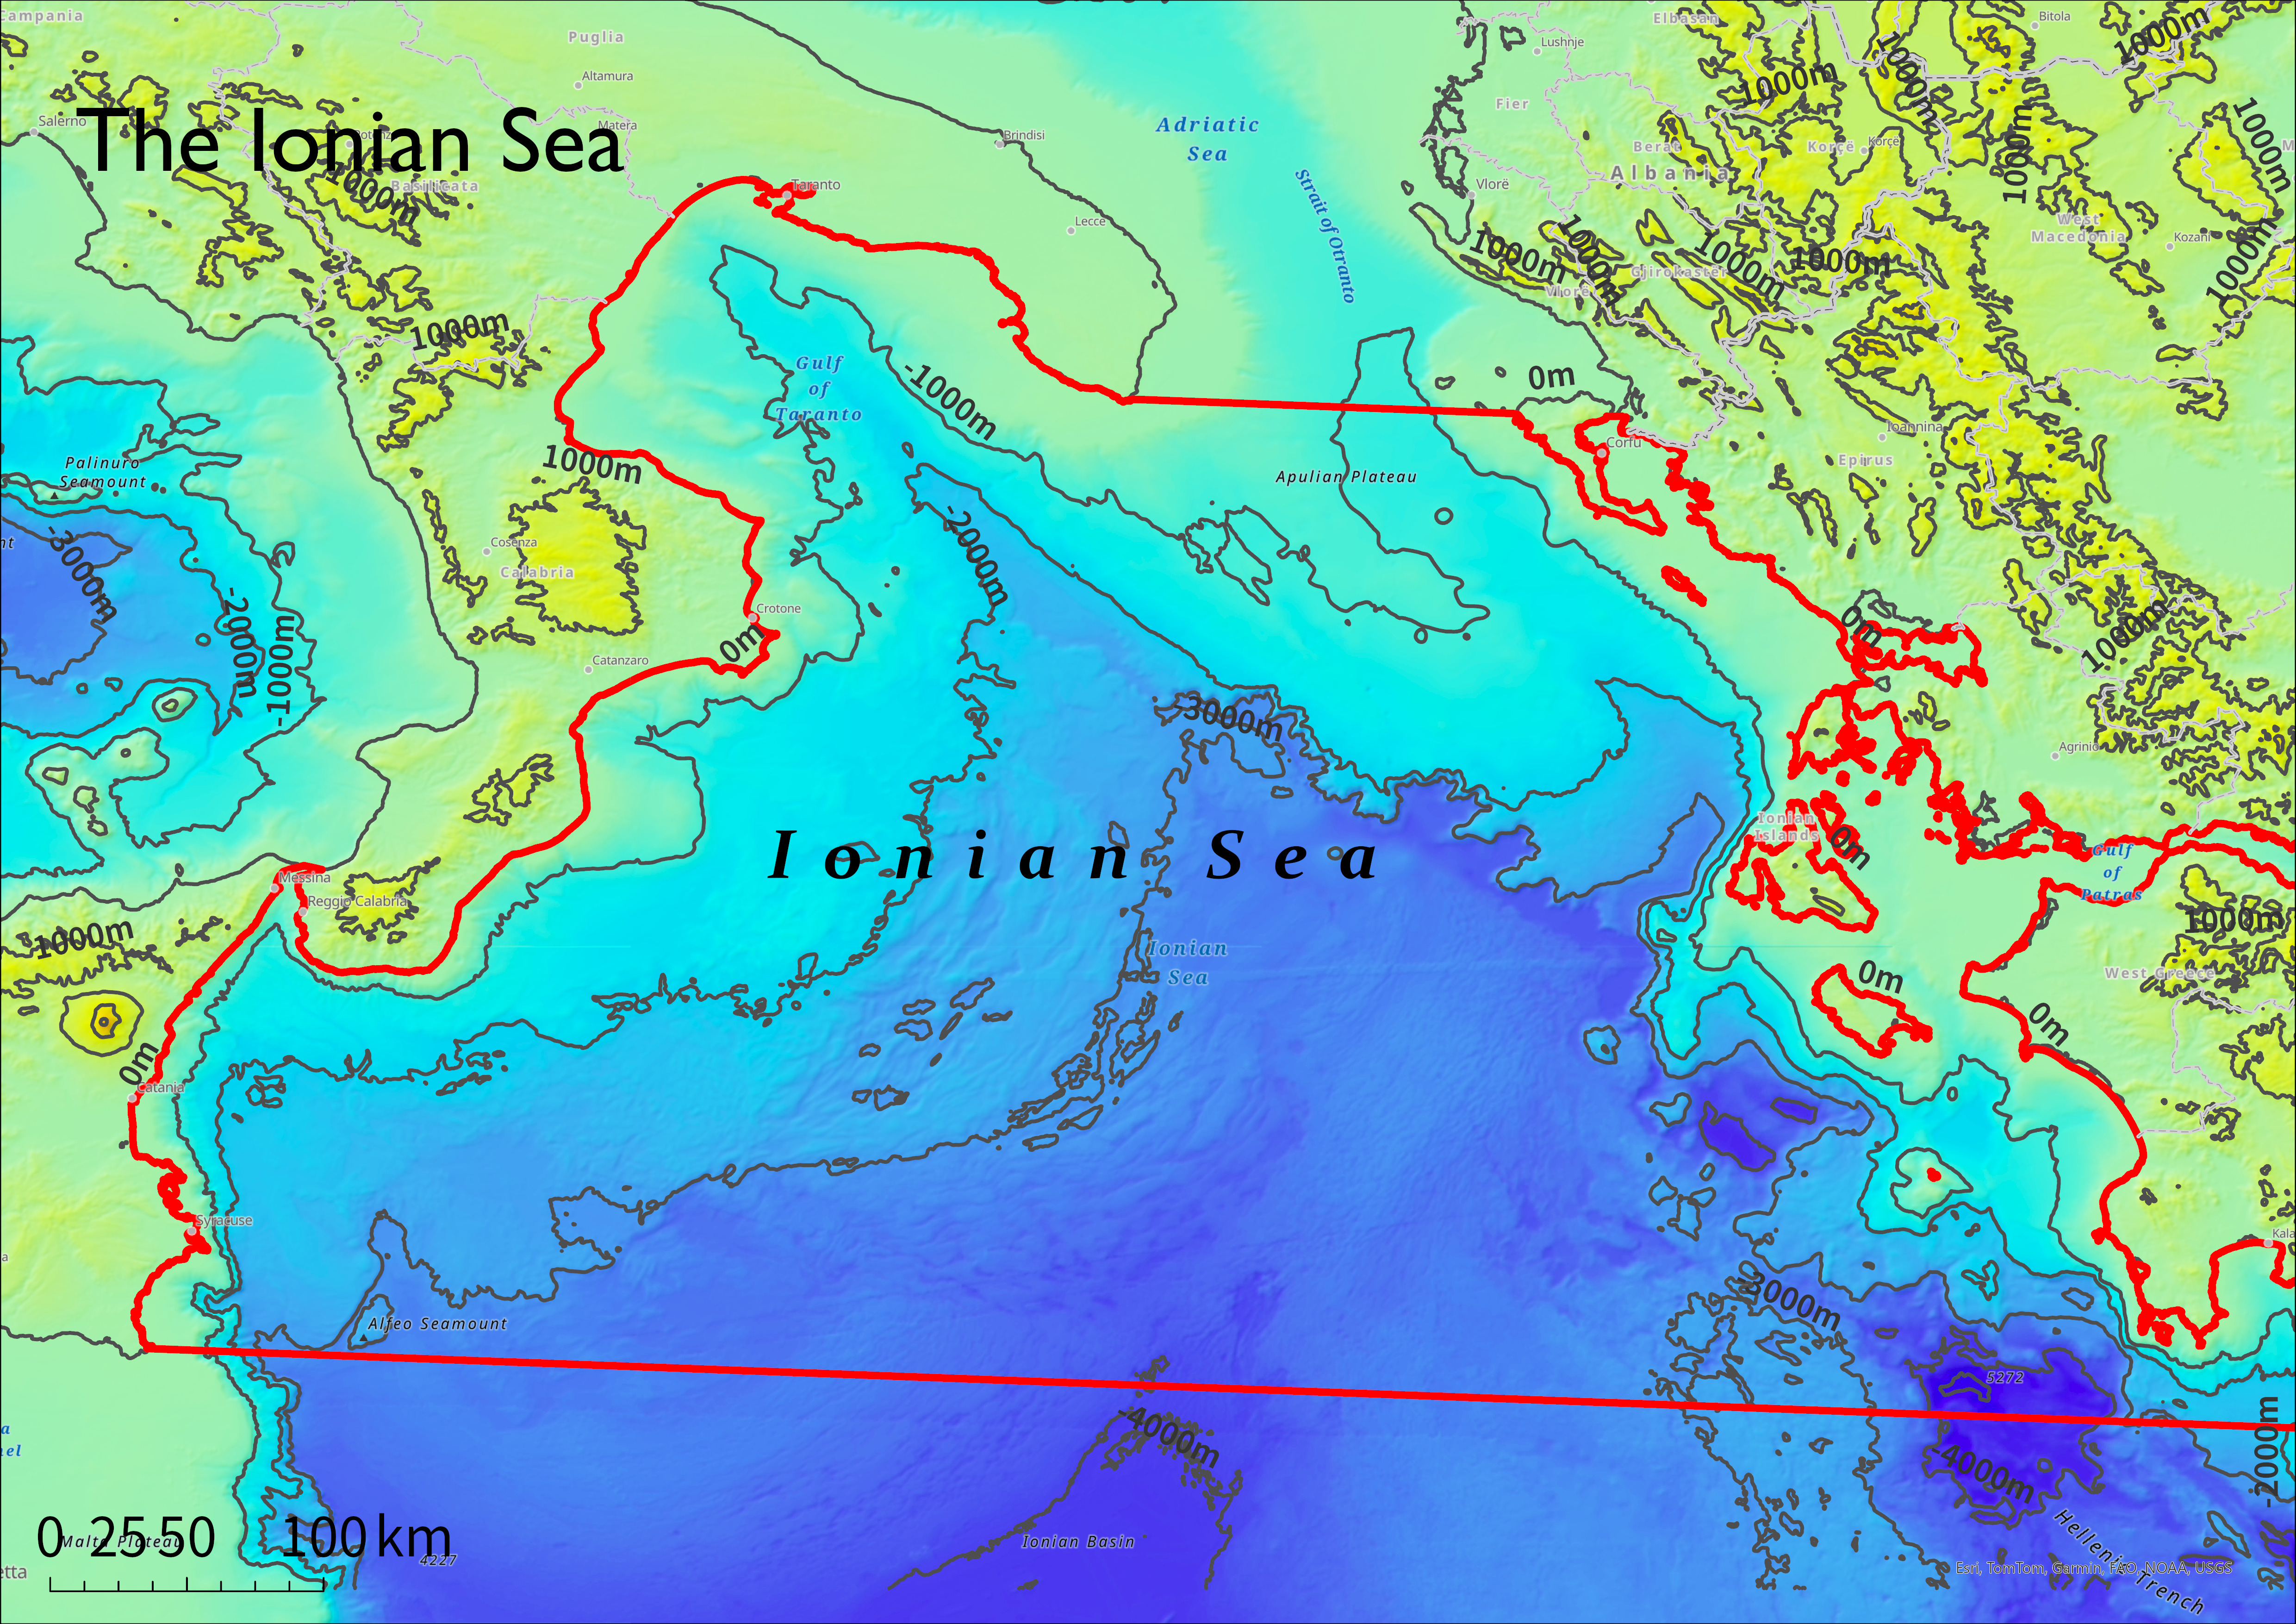
\includegraphics[width=0.5\textwidth]{fig/arcgis.jpg} \label{fig:arcgis_1}
        }
        \subfigure[Altitude across the Boundary (3D)]{
            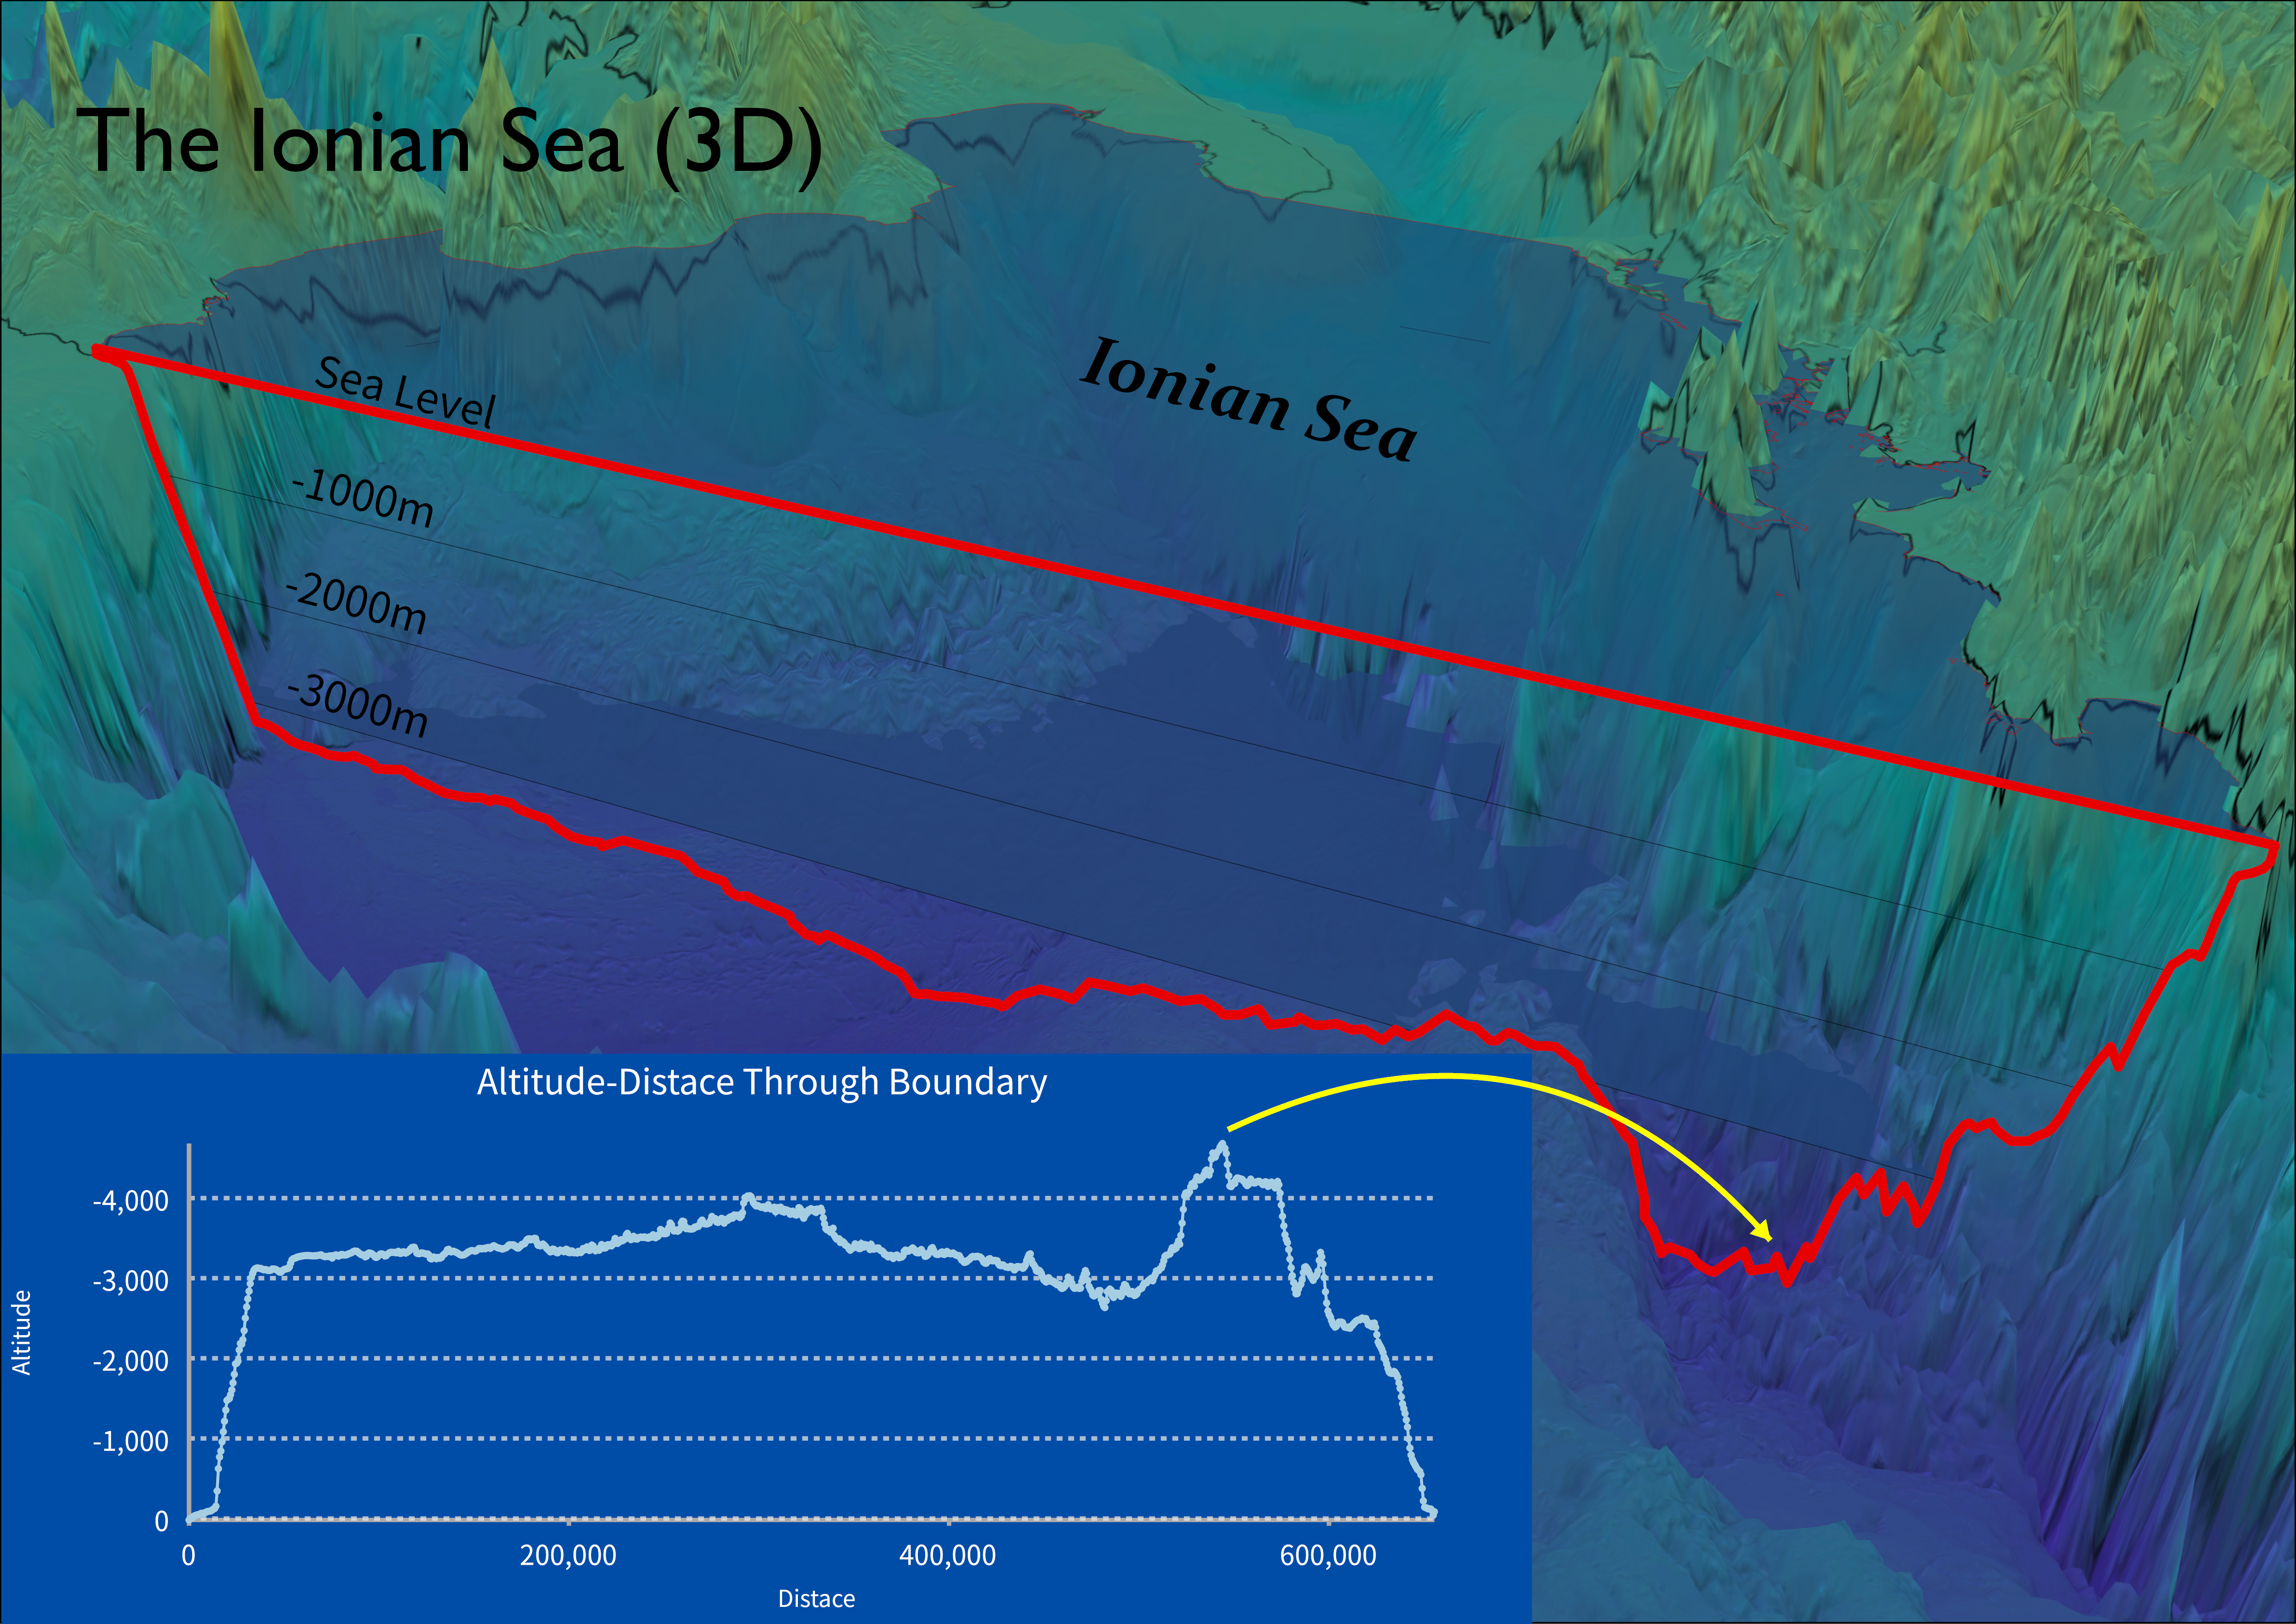
\includegraphics[width=0.5\textwidth]{fig/arcgis_1.jpg} \label{fig:arcgis_2}
        }
    }
    \caption{Data visualization using ArcGIS}
\end{figure}


Figure \ref{fig:arcgis_1} and \ref{fig:arcgis_2} show the topography and depth map of the Ionian Sea. Figure \ref{fig:arcgis_1} is two-dimensional, displaying the seabed topography using contours and indicating different depths. Figure \ref{fig:arcgis_2} is a three-dimensional view, providing a more intuitive perspective of the seabed topography. These charts display contour lines at sea level, -1000 meters, -2000 meters, and -3000 meters, and also include a cross-sectional analysis of the seabed topography.

\section{Task 1: Position Prediction Model}

\subsection{Determination of Basic Parameters of Ocean Thermodynamics}

Ocean thermodynamics is the discipline that studies the variation patterns of physical parameters such as temperature, salinity, density, etc. in the ocean and their interactions with oceanic movements. It plays a key role in the research of localization algorithms and search and rescue strategies for underwater vehicles. To carry out this research, we first need to understand some basic thermodynamic quantities, which can be elaborated in detail according to TEOS-10.

First, the oceanic pressure $p$ refers to the absolute pressure $P$ minus the standard atmospheric pressure (i.e., $P_0 = 101325Pa$). In other words, $p\equiv P-P_0$. Traditionally, absolute salinity refers to the mass fraction of dissolved substances in seawater. For seawater with a reference composition, reference salinity is currently the most reliable approximation for absolute salinity.

Based on basic thermodynamics, we can obtain the Equation \ref{eq:thermodynamics}.

\begin{equation}
    dh - \frac{1}{\rho}dp = Td\sigma + \mu dS \label{eq:thermodynamics}
\end{equation}

The thermodynamic description of seawater is crucial for understanding its behavior and characteristics. Through the Gibbs function formula, we can directly calculate various thermodynamic properties of seawater, such as entropy, specific volume, enthalpy, and potential enthalpy. The Gibbs function is described as Equation \ref{eq:gibbs}.

\begin{equation}
    g(S, \theta, p) = g^0(S, \theta, p) + \int_0^p v(S, \theta, p')dp' \label{eq:gibbs}
\end{equation}

When using the Gibbs function to determine these properties, their concepts are consistent, providing comprehensive data for understanding the thermodynamic characteristics of seawater.

In processes that do not involve heat and salinity exchange, we can assume constant entropy and salinity. Therefore, the following relationship with pressure can be used as Equation \ref{eq:enthalpy}.

\begin{equation}
    \left(\frac{\partial h}{\partial p}\right)_{S,\sigma} = \frac{1}{\rho} \label{eq:enthalpy}
\end{equation}

By integrating this equation, we can define the potential enthalpy $h^0$ as the enthalpy at the reference pressure $p_r$, as shown in Equation \ref{eq:potential_enthalpy}.

\begin{equation}
    h^0(S,\theta,p_r) = h(S,\theta,p) - \int_{p_r}^p \frac{1}{\rho(S,\theta,p')}dp' \label{eq:potential_enthalpy}
\end{equation}

Here, enthalpy and density are defined based on three state variables: salinity ($S$), potential temperature ($\theta$), and pressure ($p$).

Entropy and enthalpy play a crucial role in accurately describing the advection and diffusion of heat within the ocean. These properties are also essential for quantifying the heat exchange between the ocean, atmosphere, and ice. The Gibbs function is a function of absolute salinity, temperature, and pressure. By considering the Gibbs function, we can more accurately describe and analyze the behavior of seawater in these processes.

Using the Gibbs function for thermodynamic descriptions, we can have a more comprehensive understanding of the thermodynamic characteristics of seawater. This knowledge is crucial for various applications, including climate and ocean modeling, as well as predicting the behavior of seawater under different environmental conditions.

Therefore, as long as the temperature and salinity of the current ocean are given, together with constants, the concentration of seawater at a given location can be calculated, which plays a decisive role in the establishment of subsequent underwater dynamics models.

\subsection{Establishment of Underwater Dynamics Model}

To study the laws of motion of underwater submersibles and to determine their position and orientation, we consider that the motion of a submersible is equivalent to the motion of a rigid body in a fluid subjected to gravity and drag. The submersible is mainly affected by hydrodynamic forces (other resistance) and non-hydrodynamic forces (gravity and buoyancy). During normal motion, the submersible is mainly affected by non-hydrodynamic forces.

To model the underwater motion of the submersible, the system recommended by the International Towing Tank Conference (ITTC) and the Society of Naval Architects and Marine Engineers (SNAME) coordinate system is used to establish a reference frame and to determine various symbols. First, there is a fixed coordinate system $\xi,\eta,\zeta$, whose origin is fixed at the position where the submersible is launched, and there is also a kinematic coordinate system $x,y,z$, which moves with the submersible and whose origin is fixed at the center of gravity, G, of the submersible.


The velocity of the center of gravity of the submersible is $\vec{V}$ concerning the $x,y,z$ coordinate system, and the projection on the $x,yz,$ coordinate system is $u,v,w$. Similarly, the submersible rotates with angular velocity $\vec{\Omega}$, and the projection on the $x,y,z$ coordinate system is $p,q,r$. The external force $\vec{F}$ on the submersible is projected on the $x,y,z$ coordinate system as $X, Y, Z$; and the moment $\vec{M}$ is projected on the $x,y,z$ coordinate system as $K, M, N$. The direction of the angular velocity and the direction of the moment here follow the right-hand rule.


\begin{figure}[h!]
    \centering
    \tdplotsetmaincoords{70}{110}

    \begin{tikzpicture}[tdplot_main_coords]
        \node at (0,0,0.5) {$O$}[above];

        \draw[->] (0,0,0) -- (4,0,0) node[above] {$\xi$};
        \draw[->] (0,0,0) -- (0,5,0) node[right] {$\eta$};
        \draw[->] (0,0,0) -- (0,0,-4) node[below left] {$\zeta$};

        % draw a cylinder
        \begin{scope}[rotate around y=-25]
            \draw (2,2,-1) -- (2,5,-1);
            \draw (2,2,-3) -- (2,5,-3);
            \draw[canvas is xz plane at y=2] (2,-2) circle (1cm);
            \draw[canvas is xz plane at y=5] (2,-2) circle (1cm);

            \node at (2,3.5,-1.7) {$G$};

            \draw[-latex] (2,3.5,-2) -- (2,4.5,-2) node[above] {$X$};
            \draw[-latex] (2,3.5,-2) -- (3,3.5,-2) node[above] {$Y$};
            \draw[-latex] (2,3.5,-2) -- (2,3.5,-3) node[below left] {$Z$};

            \draw[->] (2,3.5,-2) -- (2,6.5,-2) node[above] {$x$};
            \draw[->] (2,3.5,-2) -- (8.5,3.5,-2) node[above] {$y$};
            \draw[->] (2,3.5,-2) -- (2,3.5,-4.5) node[below left] {$z$};

            \draw[-latex] (3,3.5,-4) -- (3,3.5,-4.25);
            \draw[-latex] (3,3.5,-4) -- (3,3.5,-3.75) node [left]{$r$};

            \draw[-latex] (2,5.75,-1.75) -- (2,6,-1.75);
            \draw[-latex] (2,5.75,-1.75) -- (2,5.5,-1.75) node[above] {$p$};
            \draw[-latex] (7,3.5,-1.75) -- (6.25,3.5,-1.75);
            \draw[-latex] (7,3.5,-1.75) -- (7.75,3.5,-1.75) node[above] {$q$};
            \draw[->] (1.5,3.5,-4) ++(0:1) arc (0:180:.5) node[above] {$3$};
            \draw[->, canvas is xz plane at y=2] (1.5,-1.5) ++(0:1) arc (0:-180:.5) node[above] {$1$};
            \draw[->, canvas is xz plane at y=5] (1.5,-2) ++(0:1) arc (0:180:.5) node[above] {$2$};
        \end{scope}
    \end{tikzpicture}
    \label{fig:physical_model}
    \caption{Physical model of the submersible}
\end{figure}


Figure \ref{fig:physical_model} shows the physical model of the submersible. The submersible is simplified as a capsule, and the center of gravity is marked as $G$. The $x,y,z$ coordinate system is fixed at the center of gravity of the submersible, and the $X, Y, Z$ coordinate system is fixed at the origin of the $x, y, z$ coordinate system. The $X, Y, Z$ coordinate system is the fixed coordinate system, and the $x, y, z$ coordinate system is the kinematic coordinate system.

\begin{figure}
    \centering
    \resizebox{\textwidth}{!}{
        \subfigure[The Submersible Model]{
            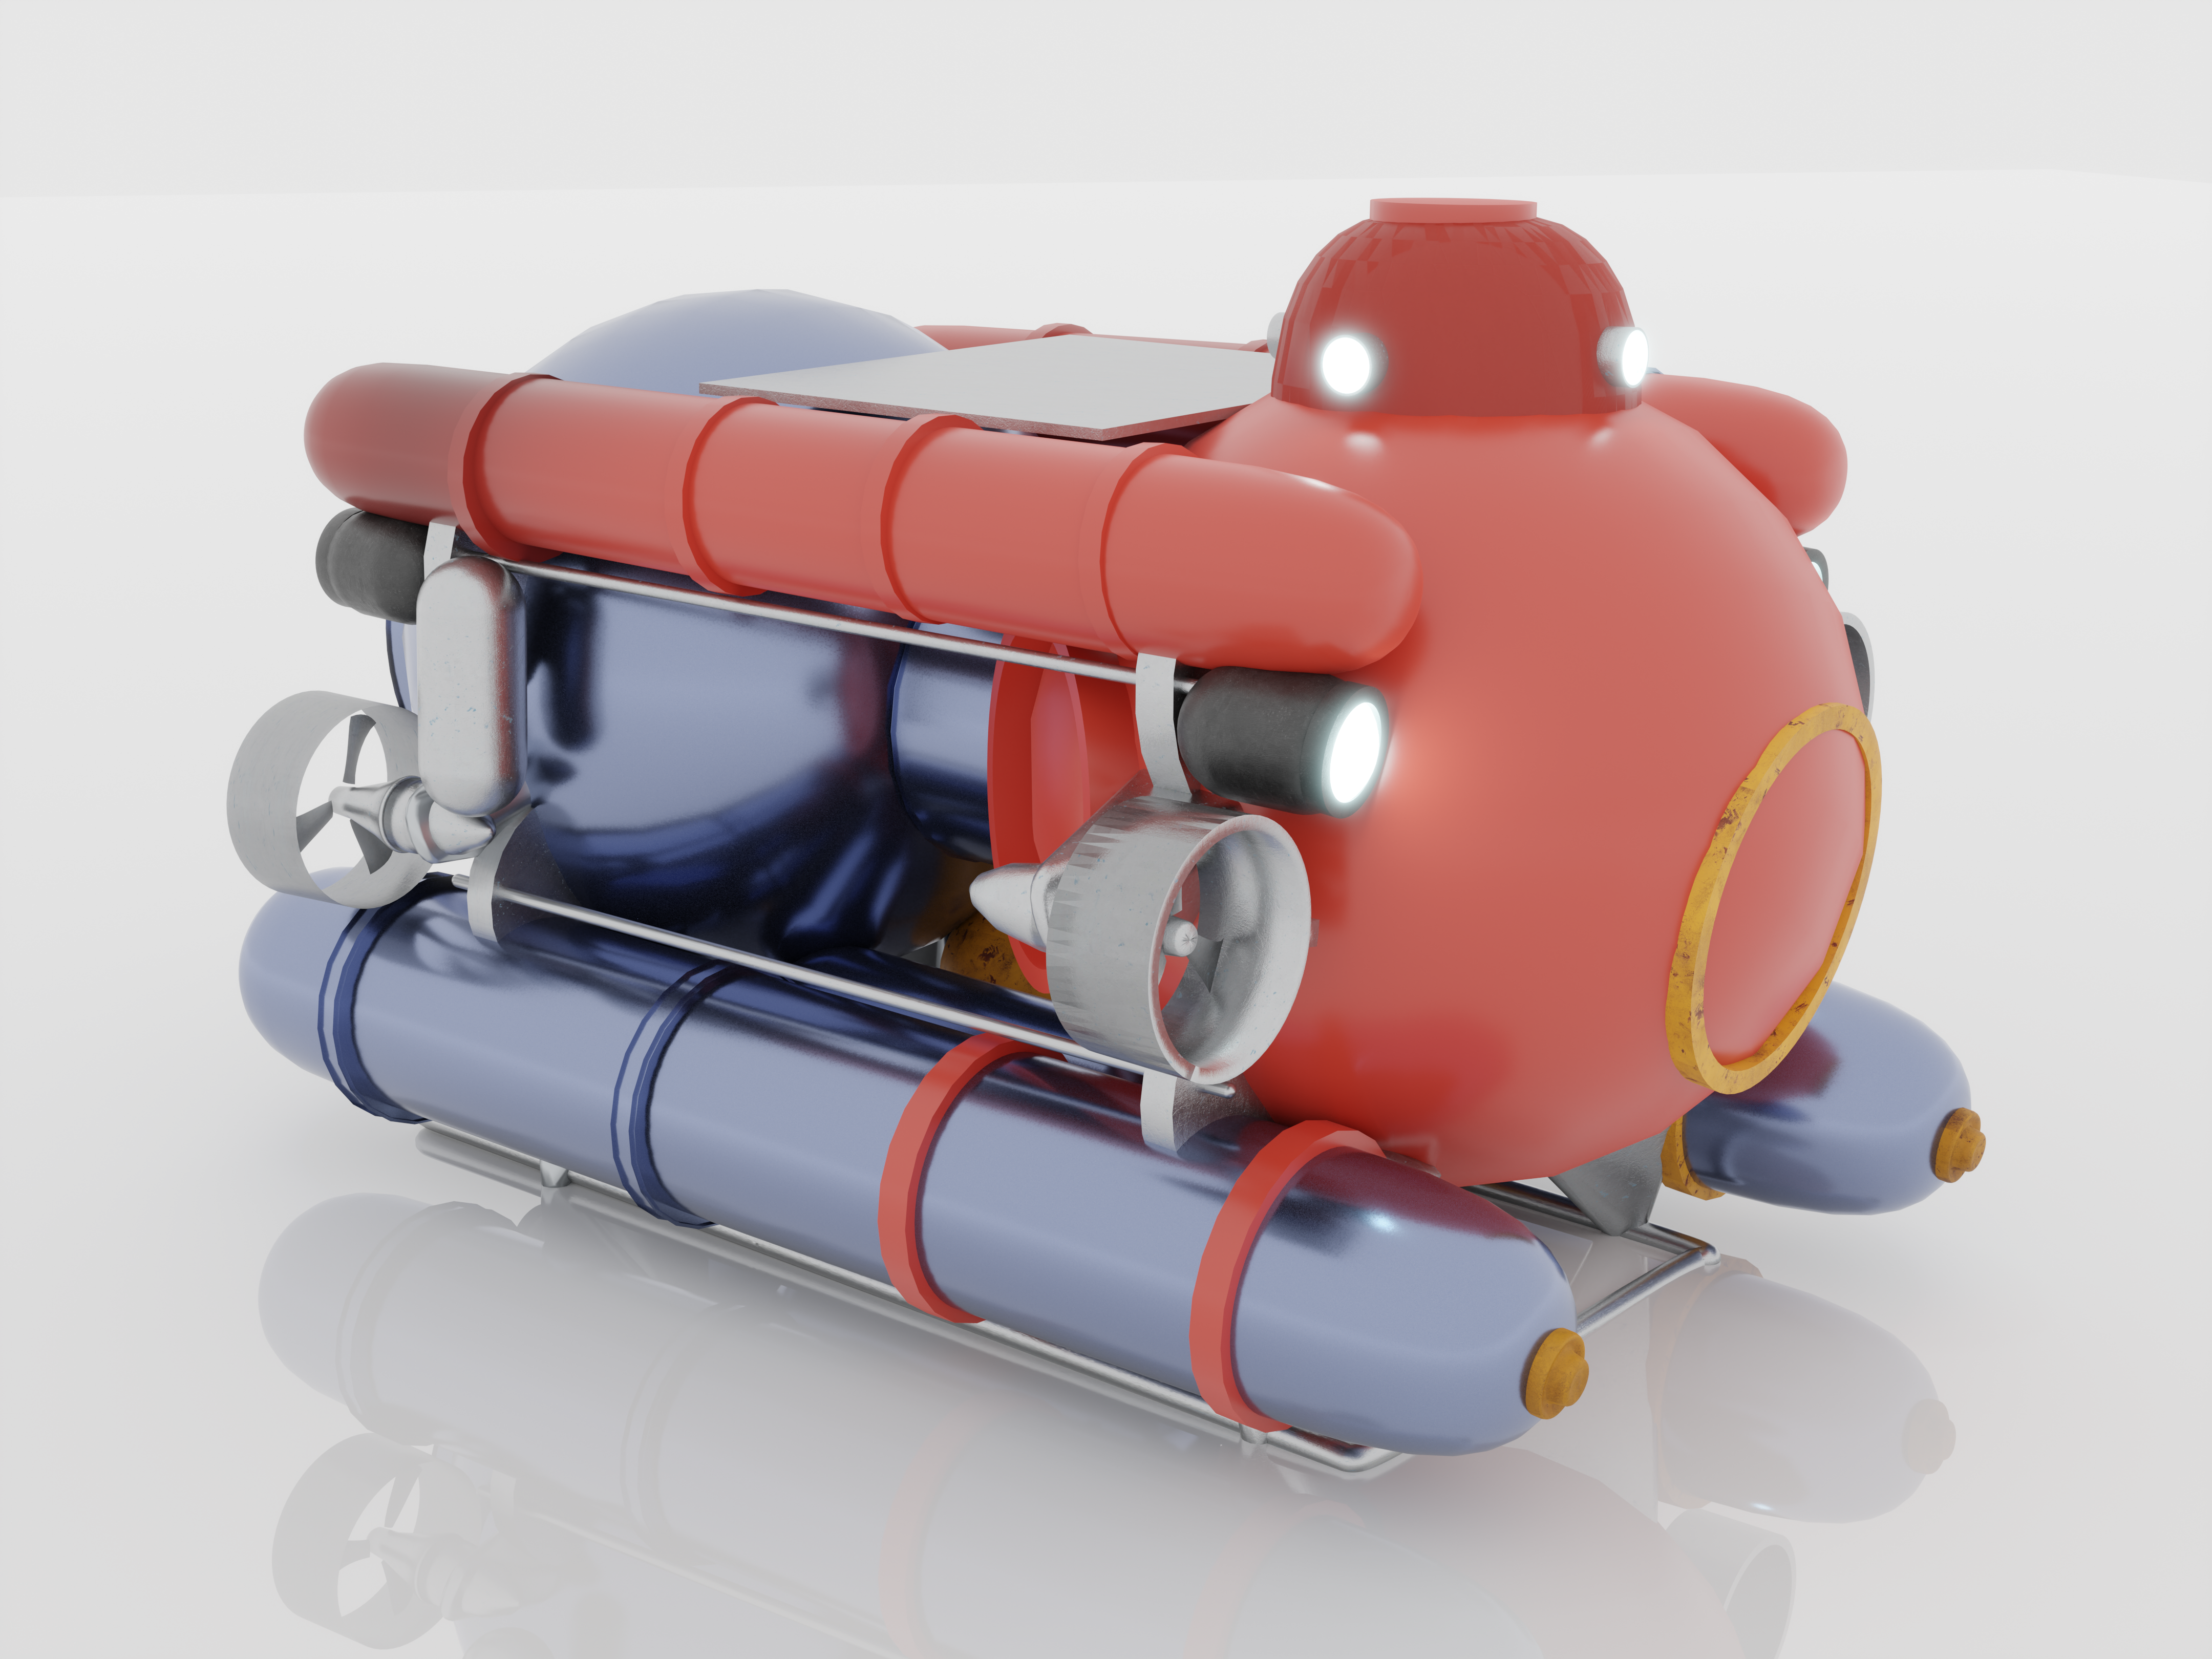
\includegraphics[width=0.5\textwidth]{fig/submersible.jpg} \label{fig:submersible}
        }
        \subfigure[The Simplified Model of the Submersible (Capsule)]{
            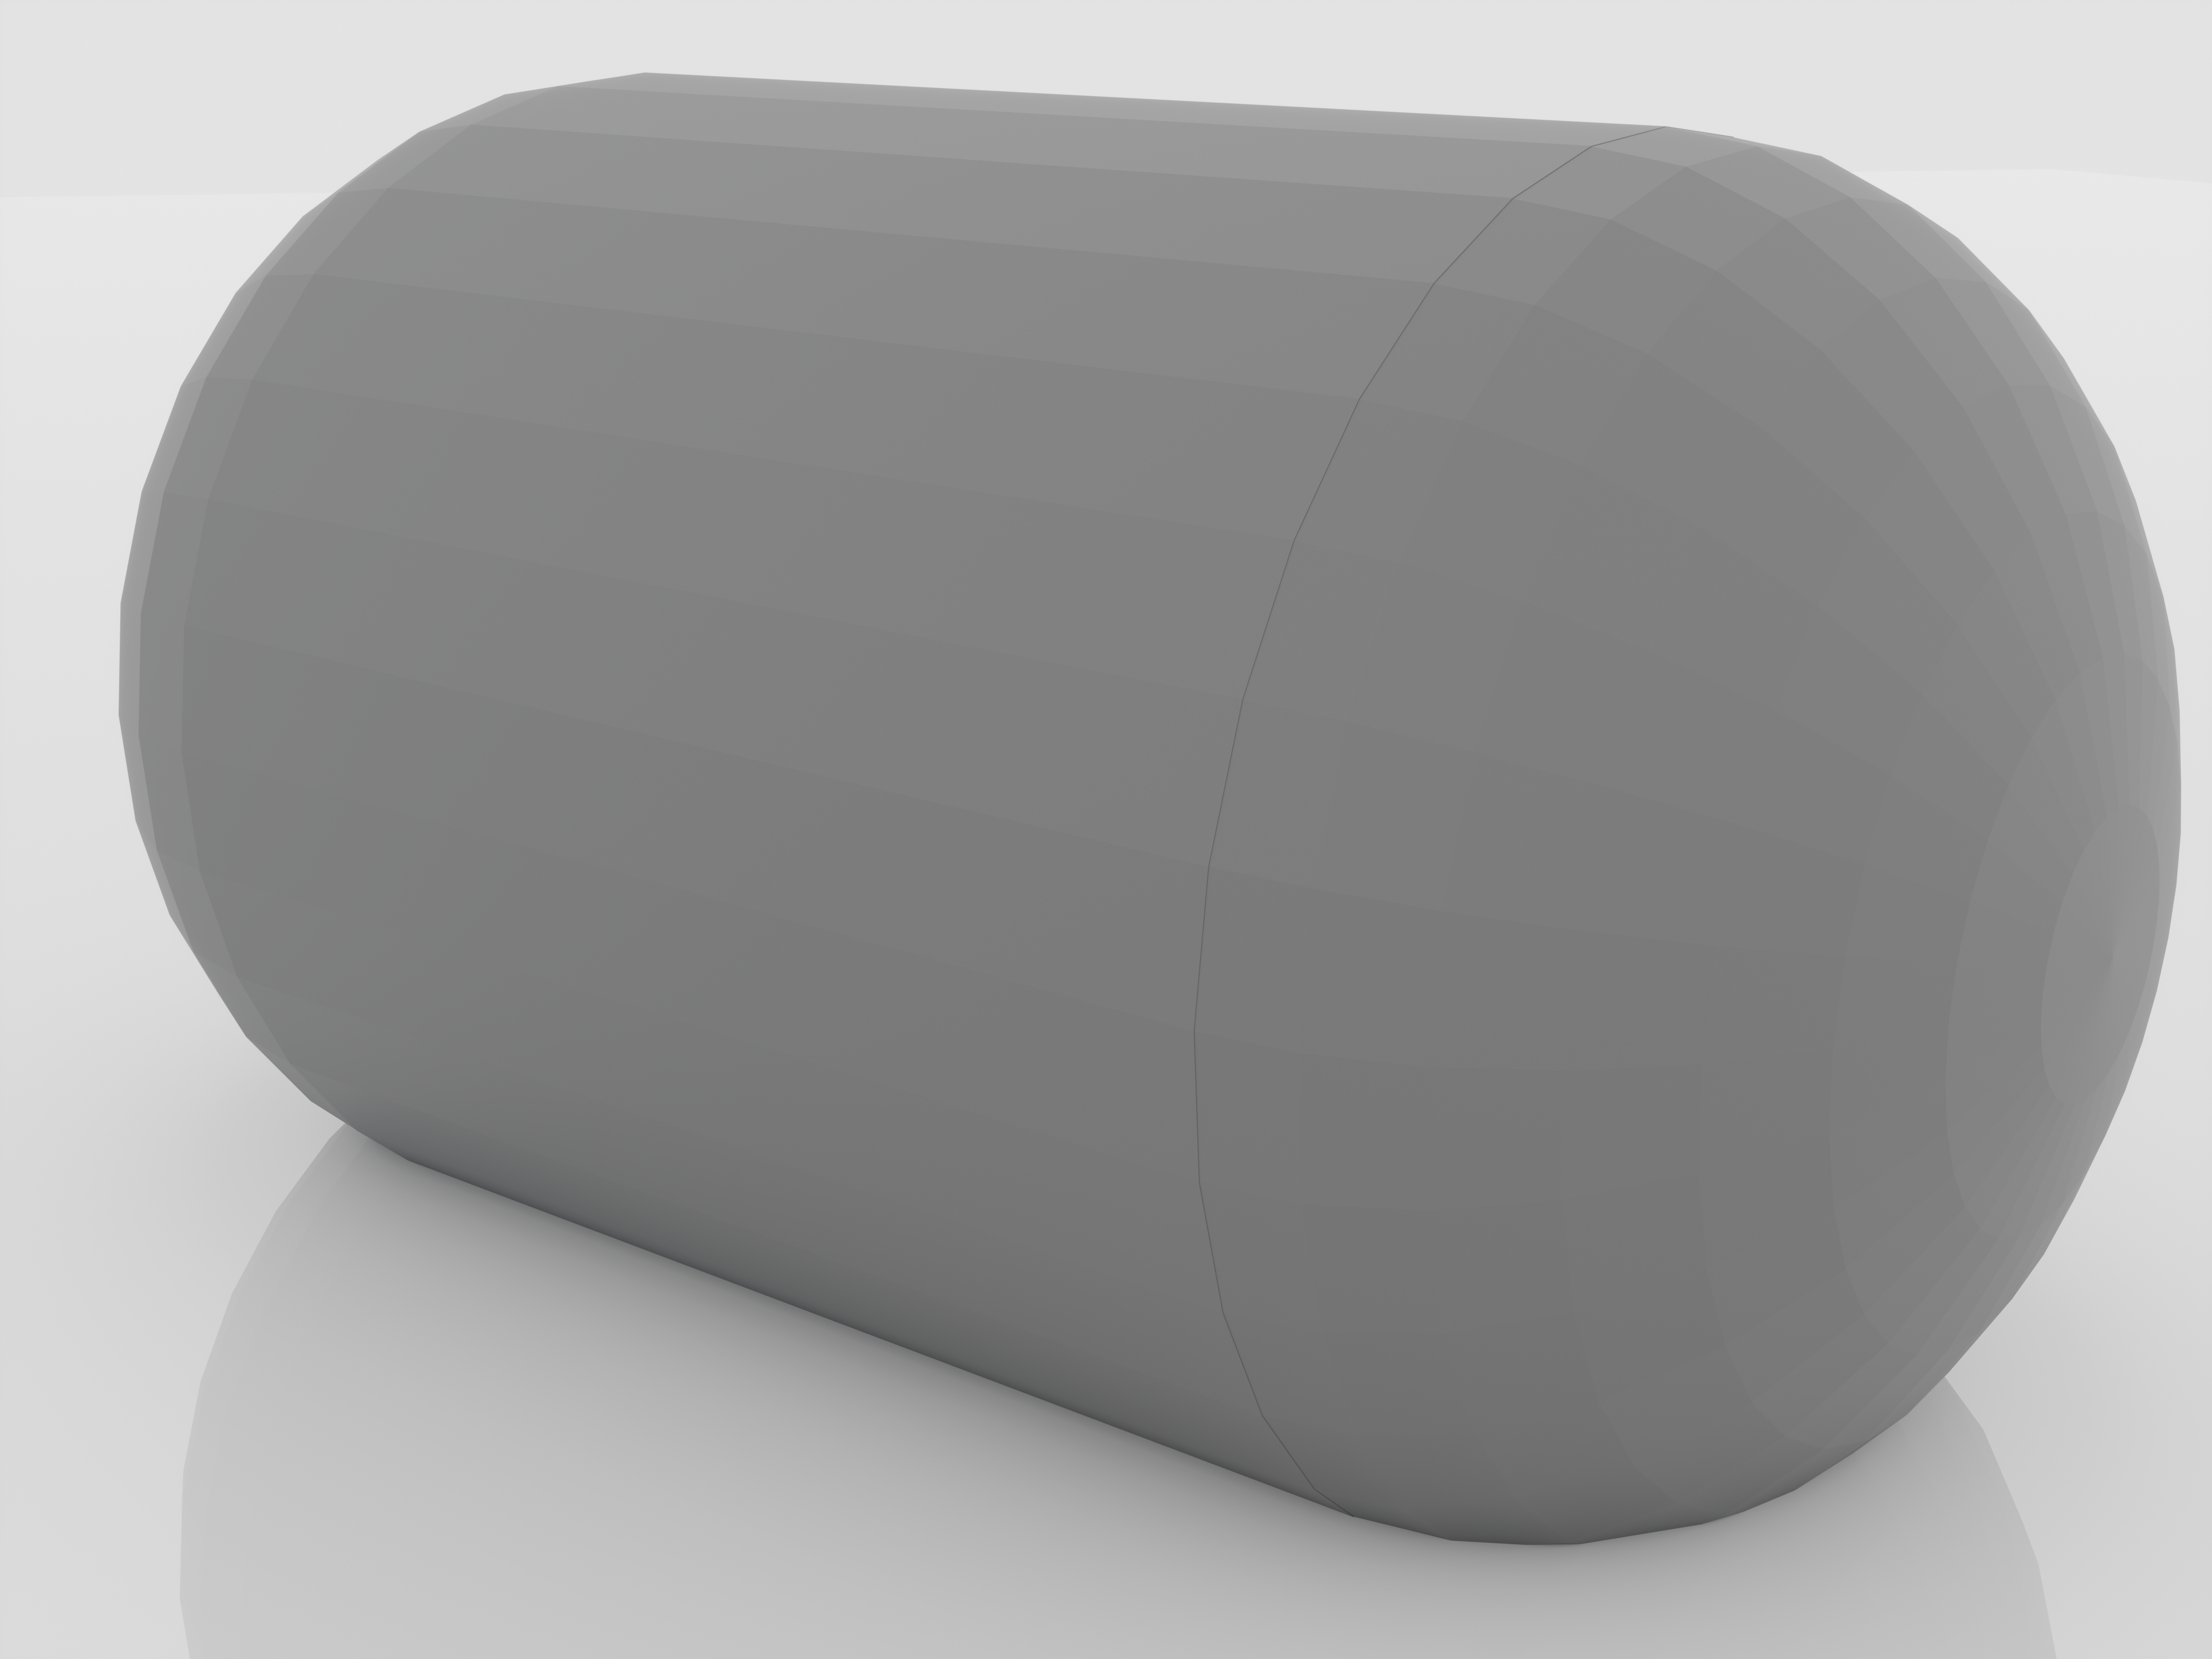
\includegraphics[width=0.5\textwidth]{fig/capsule.jpg} \label{fig:capsule}
        }
    }
\end{figure}


To simplify our model, we consider the submersible as a capsule body, as shown in Figure \ref{fig:submersible} and \ref{fig:capsule}. We assume that the mass of the submersible is $m$, the velocity of the center of gravity $G$ is $\vec{V}$, the angular velocity is $\vec{\Omega}$, the external force applied is $\vec{F}$, and the moment of the external force on the center of gravity is $\vec{M}$. According to the center of mass motion theorem and momentum moment theorem, we get the following equation:

\begin{equation}
    \left\{
    \begin{aligned}
        \frac{d\vec{B}}{dt}+\vec{\Omega}\times\vec{B}=\vec{F} \\
        \frac{d\vec{K}}{dt}+\vec{\Omega}\times\vec{K}+\vec{V}\times\vec{B}=\vec{M}
    \end{aligned}
    \right.
\end{equation}

The projection of momentum $\vec{B}=m\vec{V}$ in the kinematic coordinate system is:

\begin{equation}
    B_{x}=mu,\quad B_{y}=m\nu,\quad B_{z}=mw
\end{equation}

The equations $I_{x}, I_{y}, I_{z}$ denote the moment of inertia of the submersible concerning the axes $Gx$,$Gy$,$Gz$ of the dynamic coordinate system.
Write the above equation as a projection on the coordinate system:

\begin{equation}
    \left\{
    \begin{aligned}
        m(\dot{u}+qw-r\nu) = X   \\
        m(\dot{v}+ru-pw)=Y       \\
        m(\dot{w}+pv-qu)=Z       \\
        I_x\dot{p}+(I_z-I_y)qr=K \\
        I_y\dot{q}+(I_x-I_z)rp=M \\
        I_z\dot{r}+(I_y-I_x)pq=N
    \end{aligned}
    \right.
\end{equation}

The above six equations are the general equations for the motion of a submersible. The first three equations represent the expression of the center-of-mass motion theorem on the motion coordinate system, and the last three equations are Eulerian dynamics equations. Where $\dot{u}$ denotes the acceleration in the x-direction produced by a change in the magnitude of the velocity $u$ in the Gx-direction, and '+qw' and '-rv' are the accelerations in the x-direction due to rotation of the object with angular velocities $q$ and $r$. The other five equations are identical.
However, when studying the motion of a submersible, considering the appearance and shape of the submersible, we do not consider the motion in the transverse plane, but only in the horizontal and vertical planes. The equation of motion of the submersible on the horizontal plane is as follows:

\begin{equation}
    \left\{
    \begin{aligned}
        m(\dot{u}-r\nu) = X \\
        m(\dot{\nu}+ru)=Y   \\
        I_z\dot{r}=N
    \end{aligned}
    \right.
\end{equation}

The equation of motion of the submersible in the vertical plane is as follows:

\begin{equation}
    \left\{
    \begin{aligned}
        m(\dot{u}+qw)=X \\
        m(\dot{w}-qu)=Z \\
        I_y\dot{q}=M
    \end{aligned}
    \right.
\end{equation}

The surface of the submersible is only subjected to non-hydrodynamic forces, and the shape of the submersible is considered to be similar to that of a cylinder. To better predict the position of the diver's motion, we simplify the shape of the diver to a capsule body with volume $V_{object}$. Disregarding the steering of the vertical plane, we establish a differential equation for the velocity in the XYZ-axis direction to represent the state of motion of the submersible:

\begin{equation}
    \left\{
    \begin{aligned}
        \frac{du}{dt}=\dot{u}(t) \\
        \frac{dv}{dt}=\dot{v}(t) \\
        \frac{dw}{dt}=\dot{w}(t)
    \end{aligned}
    \right.
\end{equation}

The submersible is only affected by non-hydrodynamic forces when performing normal motion in the water, when $F_{b}=mg$. We assume that the submersible moves at a uniform speed, but the buoyancy will change due to the changes in the density and concentration of seawater, so the submersible needs to constantly adjust its evacuation volume to maintain uniform motion. The initial velocity of the submersible is set to have a magnitude of 10 m/s and a direction of southeast. The position of the submersible is recorded every $\Delta t=10s$ assuming that the equation of state of the submersible's underwater motion is:

\begin{equation}
    F_i=P(x_i,v_i,a_i)
\end{equation}

the transfer equation is

\begin{equation}
    B_i=P(x_i,v_i,a_{i+1})
\end{equation}

which gives

\begin{equation}
    F_{i+1}=F_{i}+B_{i}*\Delta t
\end{equation}

indicating that the velocity of the next state is the product of the velocity of the previous state plus the acceleration and the rate of change in time. By continuously iterating $F_i$, we can plot the variation of the diver's motion path with dive time as shown in Figure \ref{fig:variation}.

\begin{figure}[h!]
    \centering
    \includegraphics[width=.8\textwidth]{fig/variation.jpg}
    \caption{The variation of the diver's motion path with dive time}
    \label{fig:variation}
\end{figure}

\subsection{Establishment of Uncertainty Assessment Model}

A submersible may lose communication with the host vessel due to equipment damage and sink to the bottom or float at some point of neutral buoyancy. At the same time, it may be affected by environmental factors such as ocean currents, ocean density, and geographic location, and further subjected to hydrodynamic forces. Therefore, the location of the submersible is subject to uncertainty. To predict the position of a submersible, we need to model the uncertainty assessment.

\subsubsection{Ocean Currents}

Ocean currents refer to large-scale movements with relatively constant speed and direction of flow. \cite{0022-3670} Ocean currents can have a direct effect on the speed and direction of a submersible's movement. If the submersible is moving in the same direction as the current, it can utilize the power of the current to reduce its energy consumption and increase its speed. Conversely, if the submersible is moving in the opposite direction of the current, it will require more energy to overcome the resistance of the current.

The numerical prediction model we have developed about the ocean currents is based on historical records, and by statistically analyzing the data obtained from NCEI and OSCAR, we have obtained the data in Table \ref{tab:currents}, which shows that the latitudinal velocity $\vec{U}$ velocity and the meridional velocity $\vec{v}$ of the ocean currents approximately obey $N(\mu,\sigma)$. Therefore, when considering the effects of ocean currents on submersibles, we approximate the normally distributed random numbers obeying the above data as the current velocities.

\begin{figure}
    \centering
    \includegraphics[width=.8\textwidth]{fig/sea_current.jpg}
    \caption{The variation of the ocean currents}
    \label{fig:currents}
\end{figure}


\begin{table}[!h]
    \centering
    \caption{Ocean Currents Data}
    \vspace{.4cm}
    \label{tab:currents}
    \begin{tabular}{ccc}
        \toprule
        Parameters & $\displaystyle \mu $ & $\displaystyle \sigma $ \\
        \midrule
        u          & 0.01859              & 0.19707                 \\
        v          & 0.00805              & 0.16704                 \\
        \bottomrule
    \end{tabular}
\end{table}

The latitudinal velocity $\vec{U}$ velocity and meridional velocity $\vec{v}$ of the ocean current cannot be used directly in the calculation, but need to be converted as in Equation \ref{eq:uv}. before they can be substituted into our model.

\begin{equation}
    \left\{
    \begin{aligned}
        m = \sqrt{u^2+v^2} \\
        \theta = \arctan\left(\frac{v}{u}\right) \label{eq:uv}
    \end{aligned}
    \right.
\end{equation}

Where $m$ is the magnitude of the current velocity, and $\theta$ is the angle between the current velocity and the x-axis.

\subsubsection{Location Probability Model}

In the process of the submersible's movement through the water at a uniform speed, its motion is decomposed into three spatial coordinate axes. The direction of velocity is represented by $\vec{V}=[u,v,w]$, and the direction of acceleration is represented by $\vec{\dot{V}}=[\dot{u},\dot{v},\dot{w}]$. When the submersible encounters an unforeseen influence such as a power failure, the acceleration in the horizontal direction suddenly drops to zero, i.e., $\vec{\dot{V}}=[0,0,\dot{w}]$. To predict the submersible's position, we can utilize a normally distributed probability density function, expressed as Equation \ref{eq:normal_distribution}. This function is used to estimate the probability of the submersible's location, with $\mu$ representing the most likely position of the submersible and $\sigma$ determining the extent of the position probability. By discretizing the known coordinate points, we can forecast the positional probability of the submersible at the next moment.

\begin{equation}
    f_X(x)=\frac{1}{\sigma\sqrt{2\pi}}e^{\frac{-(x-\mu)^2}{2\sigma^2}} \label{eq:normal_distribution}
\end{equation}
to estimate the probability of the submersible's location. Here, $\mu$ represents the most likely position of the submersible, while $\sigma$ determines the extent of the position probability. By discretizing the known coordinate points, we can forecast the positional probability of the submersible at the next moment. Based on the mathematical Formula \ref{eq:position_probability}, we can calculate the probability of the submersible's position at the next moment.

\begin{equation}
    \sigma=\sqrt{\frac{\sum_{i=1}^n{(x_i-\overline{x})^2}}{n-1}} \label{eq:position_probability}
\end{equation}

Where $x_i$ denotes the coordinates of the known points and $\overline{x}$ indicates their mean, we can derive the variation of $\sigma$ with $\Delta t$. This variation is illustrated in the Figure. According to the empirical rule, 99.7\% of the data falls within ± three standard deviations from the mean, implying that the submersible's position is typically within these three standard deviations.

\begin{figure}[h!]
    \centering
    \includegraphics[width=.6\textwidth]{fig/variation_sigma.jpg}
    \caption{The variation of $\sigma$ with $\Delta t$}
    \label{fig:variation_sigma}
\end{figure}

Experimentally, by considering the effects of the various factors mentioned above on the submersible, we simulated the gap between the predicted trajectory and the actual trajectory and plotted the roadmap of the submersible's travel using ArcGIS software. The horizontal distance between the actual and predicted positions is represented as shown in Figure \ref{fig:trajectory}.

\begin{figure}[h!]
    \centering
    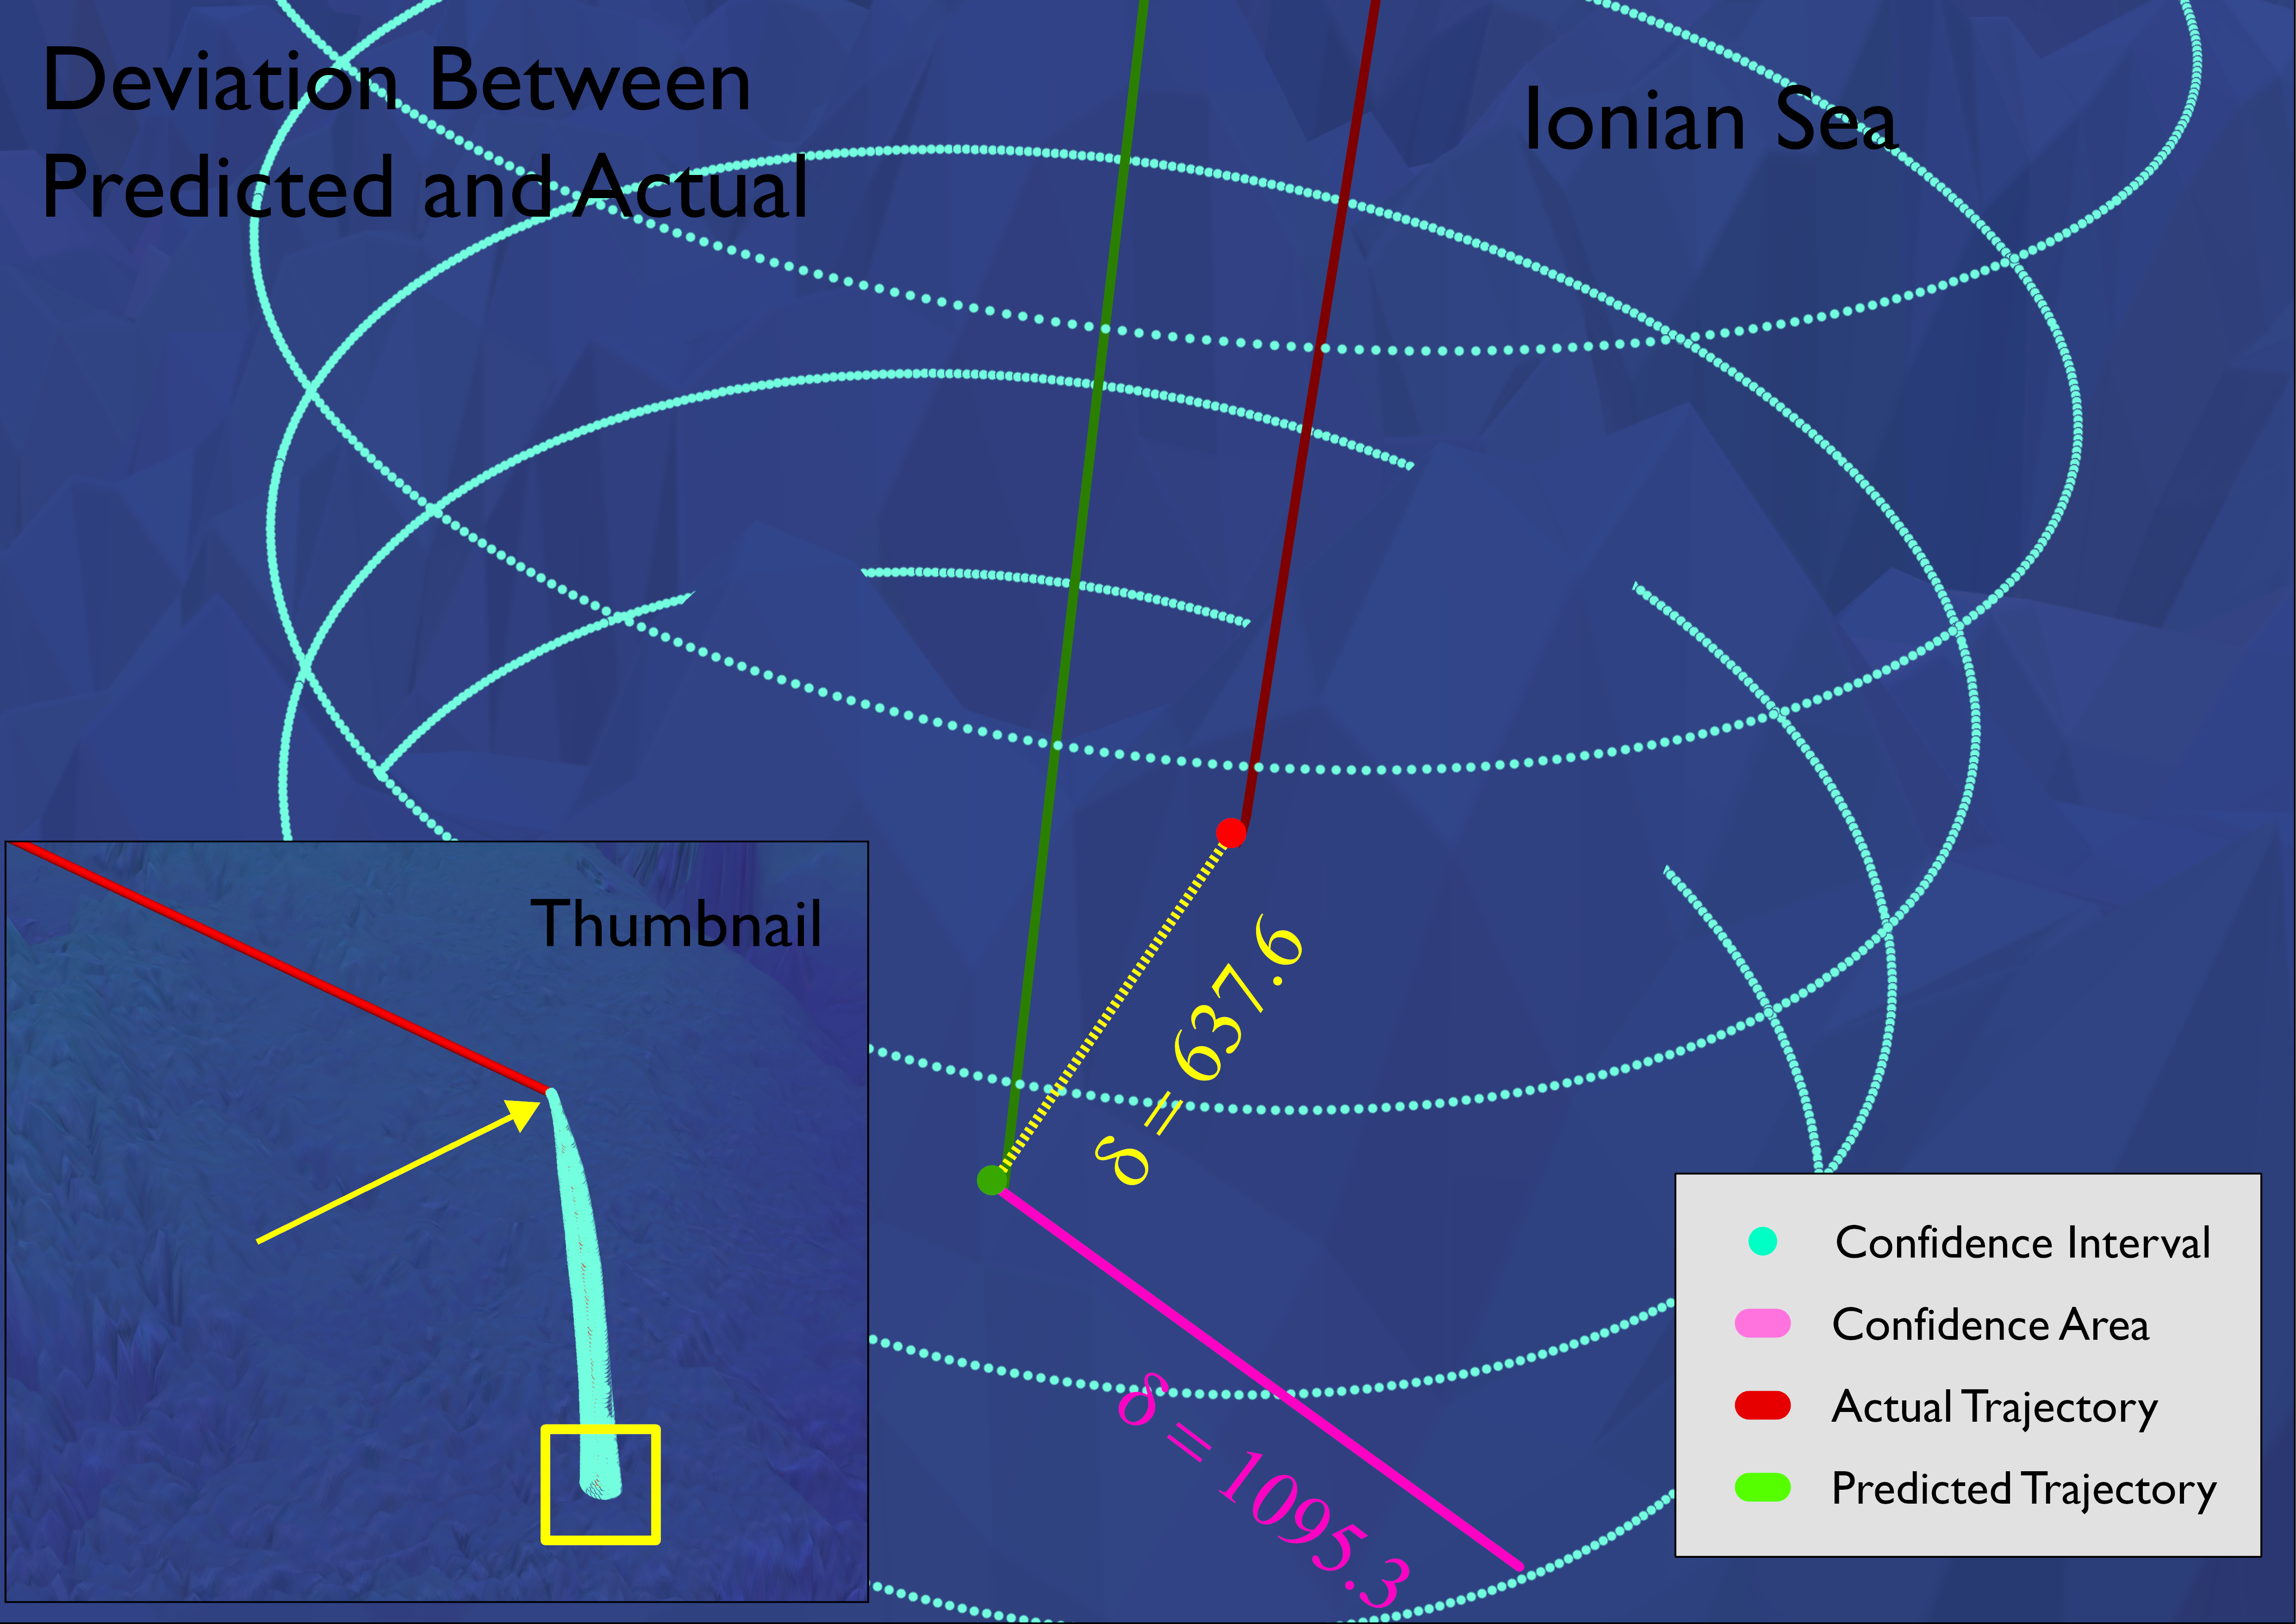
\includegraphics[width=.5\textwidth]{fig/trajectory.jpg}
    \caption{The horizontal distance between the actual and predicted positions}
    \label{fig:trajectory}
\end{figure}

Combined with the mathematical significance of the normal distribution, we use $\mu$ as the center of the circle and $3\sigma$ as the radius of the circle shown in Figure \ref{fig:2d_gaussian} to represent the probability of the possible locations of the submersible which also represents the probabilistic positional distribution of the submersible within a circle.

\begin{figure}[h!]
    \centering
    \subfigure[2D Gaussian Distribution]{
        \includegraphics[width=0.4\textwidth]{fig/2d_gaussian.png} \label{fig:2d_gaussian}
    }
    \subfigure[The variation of the submersible's position with time]{
        \includegraphics[width=0.4\textwidth]{fig/std.jpg} \label{fig:std}
    }
\end{figure}

\section{Task 2: Deployment of Search and Rescue Equipment}

\subsection{Selection of Search and Rescue Equipment}

To reduce the uncertainty factor before an accident occurs, we need to select some equipment for deployment when necessary. Considering the differences in search and rescue capabilities, maintenance costs, and preparation and utilization costs of different types of equipment, we use a comprehensive evaluation model of hierarchical analysis with entropy weighting to evaluate these equipment to ensure that the options we choose can achieve our goals.

Based on the Task \ref{problem1} model and the results obtained, we would like to have more accurate position information for each update of the submersible, so we choose the following three search devices:

\begin{itemize}
    \item \textbf{Multibeam sonar:} The acoustic wave it emits will be scattered when it hits an object in the water, and the backscattered wave will return according to its original propagation route, and then it will be received by a transducer and converted into a series of electrical impulses. By vertically arranging the received data of each emission cycle on the display, a two-dimensional acoustic map of the seafloor can be constructed, thus reflecting the characteristics of the seafloor. \cite{10.3390/rs13010035}
    \item \textbf{ROV:} As known as a Remotely Operated Underwater Vehicle (ROV), It is a remotely operated underwater robot that can dive to a depth of 3,000-10,000 meters below sea level. It is an important piece of equipment for artificial remote-controlled diving. Due to the outstanding features of ROVs such as high precision, safety, economy, high efficiency, and capability of operating at a large depth, it has been more and more widely used in the world.
    \item \textbf{AUV:} As known as an Autonomous Underwater Vehicle (AUV), it is a kind of underwater robot that can operate independently without human intervention. It is equipped with a variety of sensors and instruments, including sonar equipment, cameras, etc., for tasks such as detection and image acquisition. It can observe the behavior and distribution of marine organisms and collect relevant data to help protect the marine ecosystem and take appropriate management measures. In addition, it can perform search and rescue missions and maritime cruises, and provide services such as search and rescue of stranded persons, search for potential marine obstacles, and monitoring of marine traffic. \cite{10.1109/joe.2013.2278891}
\end{itemize}

\subsection{AHP and EWM Integrated Evaluation Model}

The evaluation indexes of this model are search and rescue capability (S), maintenance cost (M), utilization cost (U), and purchase cost (P).

\subsubsection*{Step 1: Establish the Evaluation Structure}

Through the data collection and research on these three types of equipment, we summarize the 12 evaluation indexes for measuring the optimal SAR equipment and attribute these 12 evaluation indexes to four factors: search and rescue capability, maintenance cost, usage cost, and purchase cost. The Table \ref{tab:evaluation_structure} corresponding to its hierarchy is shown below.

\begin{table}[h!]
    \centering
    \caption{Evaluation Structure}
    \label{tab:evaluation_structure}
    \vspace{.4cm}
    \resizebox{\textwidth}{!}{
        \begin{tabular}{@{}ccc@{}}
            \toprule
            Target layer                                                                                                          & Criterion layer                                    & Solution layer                               \\ \midrule
            \multirow{12}{*}{\begin{tabular}[c]{@{}c@{}}Comprehensive evaluation of search\\  and rescue equipmentA\end{tabular}} & \multirow{3}{*}{Search and rescue capability$B_1$} & Search range$C_1$                            \\
                                                                                                                                  &                                                    & Long-term search capability$C_2$             \\
                                                                                                                                  &                                                    & Positioning accuracy $C_3$                   \\ \cmidrule(l){2-3}
                                                                                                                                  & \multirow{3}{*}{Maintenance cost $B_2$}            & Repair and maintenance costs $C_4$           \\
                                                                                                                                  &                                                    & Parts supply and replacement cost $C_5$      \\
                                                                                                                                  &                                                    & Maintenance time and availability $C_6$      \\ \cmidrule(l){2-3}
                                                                                                                                  & \multirow{3}{*}{Use cost$B_3$}                     & Use training cost $C_7$                      \\
                                                                                                                                  &                                                    & Energy consumption$C_8$                      \\
                                                                                                                                  &                                                    & Data processing and analysis cost $C_9$      \\ \cmidrule(l){2-3}
                                                                                                                                  & \multirow{3}{*}{Purchase cost$B_4$}                & The price of the equipment itself is $C_10$  \\
                                                                                                                                  &                                                    & Additional equipment and sensors cost $C_11$ \\
                                                                                                                                  &                                                    & Customized demand cost $C_12$                \\ \bottomrule
        \end{tabular}
    }
\end{table}


\subsubsection*{Step 2: Establish the Judgment Matrix}

First of all, each level of indicators is analyzed to determine the weights of the indicators, that is, the indicators in the level are compared two by two, and expressed in a matrix to construct a judgment matrix. Remember this matrix $A=\left(a_{ij}\right)_{n*n}$, $a_{ij}$ represents the degree of importance (unimportance) of indicator $e_{i}$ over $e_{j}$ relative to the dominant indicator $e_{i}$ and $e_{j}$ of the dominating indicator d, indicator $e_{i}$ over $e_{j}$. The judgment matrix A satisfies:

\begin{equation}
    \left\{
    \begin{aligned}
        a_{ij}>0                                                   \\
        a_{ii}=1                                                   \\
        a_{ij}=\dfrac{1}{a_{ji}} & (i=1,2,\cdots,n;j=1,2,\cdots,n)
    \end{aligned}
    \right.
\end{equation}



\begin{equation}
    CI=\dfrac{\lambda_{max}-n}{n-1} \label{eq:CI}
\end{equation}

\begin{equation}
    CR=\dfrac{CI}{RI} \label{eq:CR}
\end{equation}

when $CI<0.1$, combined with the Equation \ref{eq:CR} we can assume that the matrix has an acceptable consistency, and the weight share of the three devices is calculated by using yaaph software.

Where the judgment matrix between the target layer and the criterion layer is shown in Table \ref{tab:judgment_matrix}.



\begin{table}[h!]

\end{table}

The consistency test result for judgment matrix A is $\lambda_{max}=0.012$. The consistency test result of judgment matrix $B_{1}$ is $\lambda_{max}=0.0279$. The consistency test for judgment matrix $B_{2}$ is $\lambda_{max}=0.0707$. The consistency test of judgment matrix $B_{3}$ is $\lambda_{max}=0.0370$. The consistency test of judgment matrix $B_{4}$ is $\lambda_{max}=0.0707$. More details are show in Table \ref{tab:judgment_matrix}, \ref{tab:judgment_matrix_1}, \ref{tab:judgment_matrix_2}, \ref{tab:judgment_matrix_3} and \ref{tab:judgment_matrix_4}.

The judgment matrix between the program level and the guideline level is shown in Table \ref{tab:judgment_matrix_2}.

\begin{figure}[ht]
    \centering
    \begin{minipage}{0.45\textwidth}
        \centering
        \caption{Judgment Matrix $A$}
        \label{tab:judgment_matrix}
        \vspace{.4cm}
        \begin{tabular}{cccccc}
            \toprule
            A       & $B_{1}$ & $B_{2}$ & $B_{3}$ & $B_{4}$ & $W_{i}$ \\
            \midrule
            $B_{1}$ & 1       & 3       & 3       & 0.25    & 0.49    \\
            $B_{2}$ & 0.33    & 1       & 1       & 0.2     & 0.13    \\
            $B_{3}$ & 0.33    & 1       & 1       & 0.25    & 0.11    \\
            $B_{4}$ & 4       & 5       & 4       & 1       & 0.27    \\
            \bottomrule
        \end{tabular}
    \end{minipage}
    \begin{minipage}{0.45\textwidth}
        \centering
        \caption{Judgment Matrix $B_{1}$}
        \label{tab:judgment_matrix_1}
        \vspace{.4cm}
        \begin{tabular}{ccccc}
            \toprule
            $B_{1}$ & $C_{1}$ & $C_{2}$ & $C_{3}$ & $W_{i}$ \\
            \midrule
            $C_{1}$ & 1       & 0.2     & 0.33    & 0.11    \\
            $C_{2}$ & 5       & 1       & 1       & 0.48    \\
            $C_{3}$ & 3       & 1       & 1       & 0.40    \\
            \bottomrule
        \end{tabular}
    \end{minipage}
    \begin{minipage}{0.45\textwidth}
        \centering
        \caption{Judgment Matrix $B_{2}$}
        \label{tab:judgment_matrix_2}
        \vspace{.4cm}
        \begin{tabular}{ccccc}
            \toprule
            $B_{2}$ & $C_{4}$ & $C_{5}$ & $C_{6}$ & $W_{i}$ \\
            \midrule
            $C_{4}$ & 1       & 0.33    & 3       & 0.27    \\
            $C_{5}$ & 3       & 1       & 5       & 0.12    \\
            $C_{6}$ & 0.33    & 0.2     & 1       & 0.61    \\
            \bottomrule
        \end{tabular}
    \end{minipage}
    \begin{minipage}{0.45\textwidth}
        \centering
        \caption{Judgment Matrix $B_{3}$}
        \label{tab:judgment_matrix_3}
        \begin{tabular}{ccccc}
            \toprule
            $B_{3}$ & $C_{7}$ & $C_{8}$ & $C_{9}$ & $W_{i} $ \\
            \midrule
            $C_{7}$ & 1       & 3       & 0.33    & 0.26     \\
            $C_{8}$ & 0.33    & 1       & 0.25    & 0.64     \\
            $C_{9}$ & 3       & 4       & 1       & 0.10     \\
            \bottomrule
        \end{tabular}
    \end{minipage}
    \begin{minipage}{0.45\textwidth}
        \centering
        \caption{Judgment Matrix $B_{4}$}
        \label{tab:judgment_matrix_4}
        \vspace{.4cm}
        \begin{tabular}{ccccc}
            \toprule
            $B_{4}$  & $C_{10}$ & $C_{11}$ & $C_{12}$ & $W_{i}$ \\
            \midrule
            $C_{10}$ & 1        & 0.33     & 3        & 0.27    \\
            $C_{11}$ & 3        & 1        & 4        & 0.12    \\
            $C_{12}$ & 0.33     & 0.25     & 1        & 0.61    \\
            \bottomrule
        \end{tabular}
    \end{minipage}
    \begin{minipage}{0.45\textwidth}
        \centering
        \caption{Weight Share of Each Selected Device}
        \label{tab:weight_share}
        \begin{tabular}{ccc}
            \toprule
            Multibeam Radar & ROV    & AUV    \\ \midrule
            0.2161          & 0.2716 & 0.5133 \\ \bottomrule
        \end{tabular}
    \end{minipage}
\end{figure}

Therefore, we can derive the weight share of each selected device as Table \ref{tab:weight_share}.

Due to the high subjectivity of the hierarchical analysis method, to make the results more correct, we use the entropy weight method to further improve the model. For the optimal equipment selection evaluation system, synthesizing the hierarchical analysis method we have the following $m \times n$ matrix in Table \ref{tab:entropy_weight_matrix}.

\begin{table}[h!]
    \centering
    \caption{Entropy Weight Matrix}
    \label{tab:entropy_weight_matrix}
    \vspace{.4cm}
    \begin{tabular}{ccccc}
        \toprule
        Category         & S      & M      & U      & P      \\
        \midrule
        Multi-beam Sonar & 0.3274 & 0.2190 & 0.4784 & 0.1030 \\
        ROV              & 0.1996 & 0.3712 & 0.2222 & 0.2996 \\
        AUV              & 0.4729 & 0.4098 & 0.2994 & 0.5974 \\
        \bottomrule
    \end{tabular}
\end{table}

% Firstly, the data is dimensionless. The optimal value of each column in the matrix is represented as follows:

% \begin{equation}
%     r_j^*=
%     \begin{cases}
%         \max_ir_{ij}, & \text{if $j$represents a profitability indicator} \\\min_ir_{ij},&\text{if $j$represents a cost-based indicator}
%     \end{cases},\quad i=1,2,\ldots,m;\quad j=1,2,\ldots,n;
% \end{equation}

% Next, the data is normalized, and the matrix is denoted as:

% \begin{equation}
%     S = (s_{ij})_{m \times n},
% \end{equation}

% where

% \begin{equation}
%     r_j^* = \begin{cases}
%         \underset{i}{\max} r_{ij}, & \text{if $j$ represents a profitability indicator} \\
%         \underset{i}{\min} r_{ij}, & \text{if $j$ represents a cost-based indicator}
%     \end{cases}, \quad i = 1,2,\ldots, m; \quad j = 1, 2, \ldots, n;
% \end{equation}

The matrix S is then normalized, and the entropy of the $j$th evaluation indicator is defined as:

\begin{equation}
    H_j = -k\sum_{i=1}^m t_{ij}\ln t_{ij}, \quad (j = 1, 2, \ldots, n),
\end{equation}

where $t_{ij} = \frac{s_{ij}}{\sum_{i=1}^{m}s_{ij}^{'}}$, $j = 1, 2, \ldots, n$, and $k = \frac{1}{\ln m}$. The coefficient of variation for the $j$th evaluation metric is calculated as:

\begin{equation}
    \alpha_j = 1 - H_j, \quad (j = 1, 2, \ldots, n).
\end{equation}

The entropy weight for the $j$th evaluation metric is defined as:

\begin{equation}
    \omega_j = \frac{\alpha_j}{\sum_{j=1}^n\alpha_j}, \quad (j = 1, 2, \ldots, n),
\end{equation}

and it satisfies the conditions $0 \leq \omega_j \leq 1$ and $\sum_{j=1}^n\omega_j = 1$. According to the entropy weighting method, the weights of the indicators are $\lambda$ = [0.25, 0.23, 0.24, 0.28]. By integrating the evaluation methods, the evaluation result of the $j$th evaluation method for the $i$th evaluation object is denoted as $y_{ij}$. Using the weighting idea, we introduce the following model:

\begin{equation}
    \hat{y_i} = f(y_{ij},\lambda_j), \quad (i = 1,2,\ldots,m),
\end{equation}

where $\hat{y_i}$ is the integrated evaluation result for the $i$th evaluation object, $\lambda_j$ is the relative weight of the $j$th evaluation method, and $f$ is the integrated model of the evaluation method. The entropy weight of the three devices is calculated as Table \ref{tab:entropy_weight}.

\begin{table}[h!]
    \centering
    \caption{Entropy Weight of Each Selected Device}
    \vspace{.4cm}
    \label{tab:entropy_weight}
    \begin{tabular}{ccc}
        \toprule
        Multibeam Radar & ROV    & AUV    \\ \midrule
        0.1850          & 0.2808 & 0.5342 \\ \bottomrule
    \end{tabular}
\end{table}

After calculation, we derived the weights for subjective and objective evaluation by hierarchical analysis and entropy weighting. After considering the search and rescue capability, the cost of use and maintenance, and the cost of purchase, we concluded that the AUV could be deployed on the main ship.

\section{Task 3: Search for the Missing Submersible}

\subsection{State of the Submersible Underwater}

Through our modeling, we have determined that there are two states in which a lost-feeding submersible exists underwater:

\begin{itemize}
    \item The submersible stops feeding and therefore has a high probability of floating in an area of the ocean.
    \item The submersible takes on too much water and floats in an area of the ocean and then sinks to the bottom of the ocean.
\end{itemize}

\subsection{Determination of Search and Rescue Mode}

After determining the two possible states of a lost submersible underwater, we used the submersible underwater dynamics model to build a probabilistic model diagram of a lost submersible underwater. The model diagram is approximated as a positive circular table shape with the radius of the upper bottom surface as $r$ and the radius of the lower bottom surface as $R$. Based on this model, we determined the search and rescue model.

\begin{itemize}
    \item First, we let the AUV start from the center of the circle on the surface of the dome where the diver was lost and dive along the predicted route directly to the end of the predicted roadmap, i.e., the center of the circle on the bottom surface under the predicted dome. This is because the probability of the lost submersible being on that path is the highest, as shown in Figure \ref{fig:step1}.
    \item We then allowed the AUV located on the bottom to spiral up to the surface and, over time, set the final AUV drop point at the $r/2$ position of the bottom surface of the round table, as shown in Figure \ref{fig:step2}.
    \item When the AUV reaches the surface, we again let the AUV spiral down to the bottom. This time, we kept the radius of the spiral the same so that the AUV landed at position $r/4$ on the bottom surface under the circular platform, as shown in Figure \ref{fig:step3}.
    \item We again let the AUV follow the spiral up and over time, so that the submersible reaches the rounded edge of the bottom surface, as shown in Figure \ref{fig:step4}.
    \item We repeat step 3 and let the AUV sink following a spiral and with time the radius increases as it sinks but does not reach the rounded edge of the lower bottom surface, as shown in Figure \ref{fig:step5}.
\end{itemize}

Since then, with these steps, we can cover the entire circular table as well as the detection radius of the AUV.

\begin{figure}[h!]
    \centering
    \subfigure[Step 1]{
        \includegraphics[width=0.3\textwidth]{fig/plot1.png.jpg} \label{fig:step1}
    }
    \subfigure[Step 2]{
        \includegraphics[width=0.3\textwidth]{fig/plot2.png.jpg} \label{fig:step2}
    }
    \subfigure[Step 3]{
        \includegraphics[width=0.3\textwidth]{fig/plot3.png.jpg} \label{fig:step3}
    }
    \subfigure[Step 4]{
        \includegraphics[width=0.3\textwidth]{fig/plot4.png.jpg} \label{fig:step4}
    }
    \subfigure[Step 5]{
        \includegraphics[width=0.3\textwidth]{fig/plot5.png.jpg} \label{fig:step5}
    }
    \caption{Search and Rescue Model}
    \label{fig:search_rescue}
\end{figure}

% 搜救模式及模型的可行性
\subsubsection{Feasibility of the Search and Rescue Model}

Through the experimental verification of the above model, and substituting the shortest path algorithm and the idea of greed, we can traverse the whole probability model

At this point, we analyze the probability model, which will be divided into n circles with the circular platform, the lost diver exists in the center of each circle is the largest probability, and the farther away from the center of the circle, the probability gradually decreases and the probability is unlikely to be zero, which can be seen, the probability of the lost diver in the circle in line with the normal distribution.

Let $3σ$ be the radius of any circle, the probability that the lost submersible is within the circle is 99.74\%. All circles obey this law, and it is statistically significant that the probability of a lost diver being within this circle is also 99.74\%. This shows that the feasibility of this model is extremely high.

\begin{figure}
    \centering
    \includegraphics[width=.4\textwidth]{fig/possibility.jpg}
    \caption{Feasibility of the Search and Rescue Model}
    \label{fig:feasibility}
\end{figure}


\section{Task 4: Model Extension and Multi-Objective Problem}

\subsection{Other Tourist Areas}

To improve the generalizability of the model, we extend the location prediction model to other tourist destinations and consider the effect of simultaneous movements of multiple submersibles on the model.

\textbf{Differences in environmental parameters:} Taking the Caribbean Sea as an example, there are significant differences between the Caribbean Sea and the Ionian Sea in terms of physical factors such as ocean concentration, seawater density, current speed, and seabed conditions. In our model, the effects of these parameters on the predicted positions are taken into account, and we achieve the goal of predicting the position of the submersible in each location by varying these parameters.

\textbf{How the model was modified:} For the Caribbean Sea application, we downloaded the data of ocean elevation, seawater temperature, current velocity, and absolute salinity from GEBCO and processed the data. Using the data visualization function of AirGIS, we obtained an image of the position of the submersible in the Caribbean Sea.

\textbf{Promote the modified model:} Based on the established model, we only have various physical parameters of the ocean, such as ocean density and seawater concentration, and we can extend the model to all regions.

\begin{figure}[h!]
    \centering
    \subfigure[The Position of the Submersible in the Caribbean Sea]{
        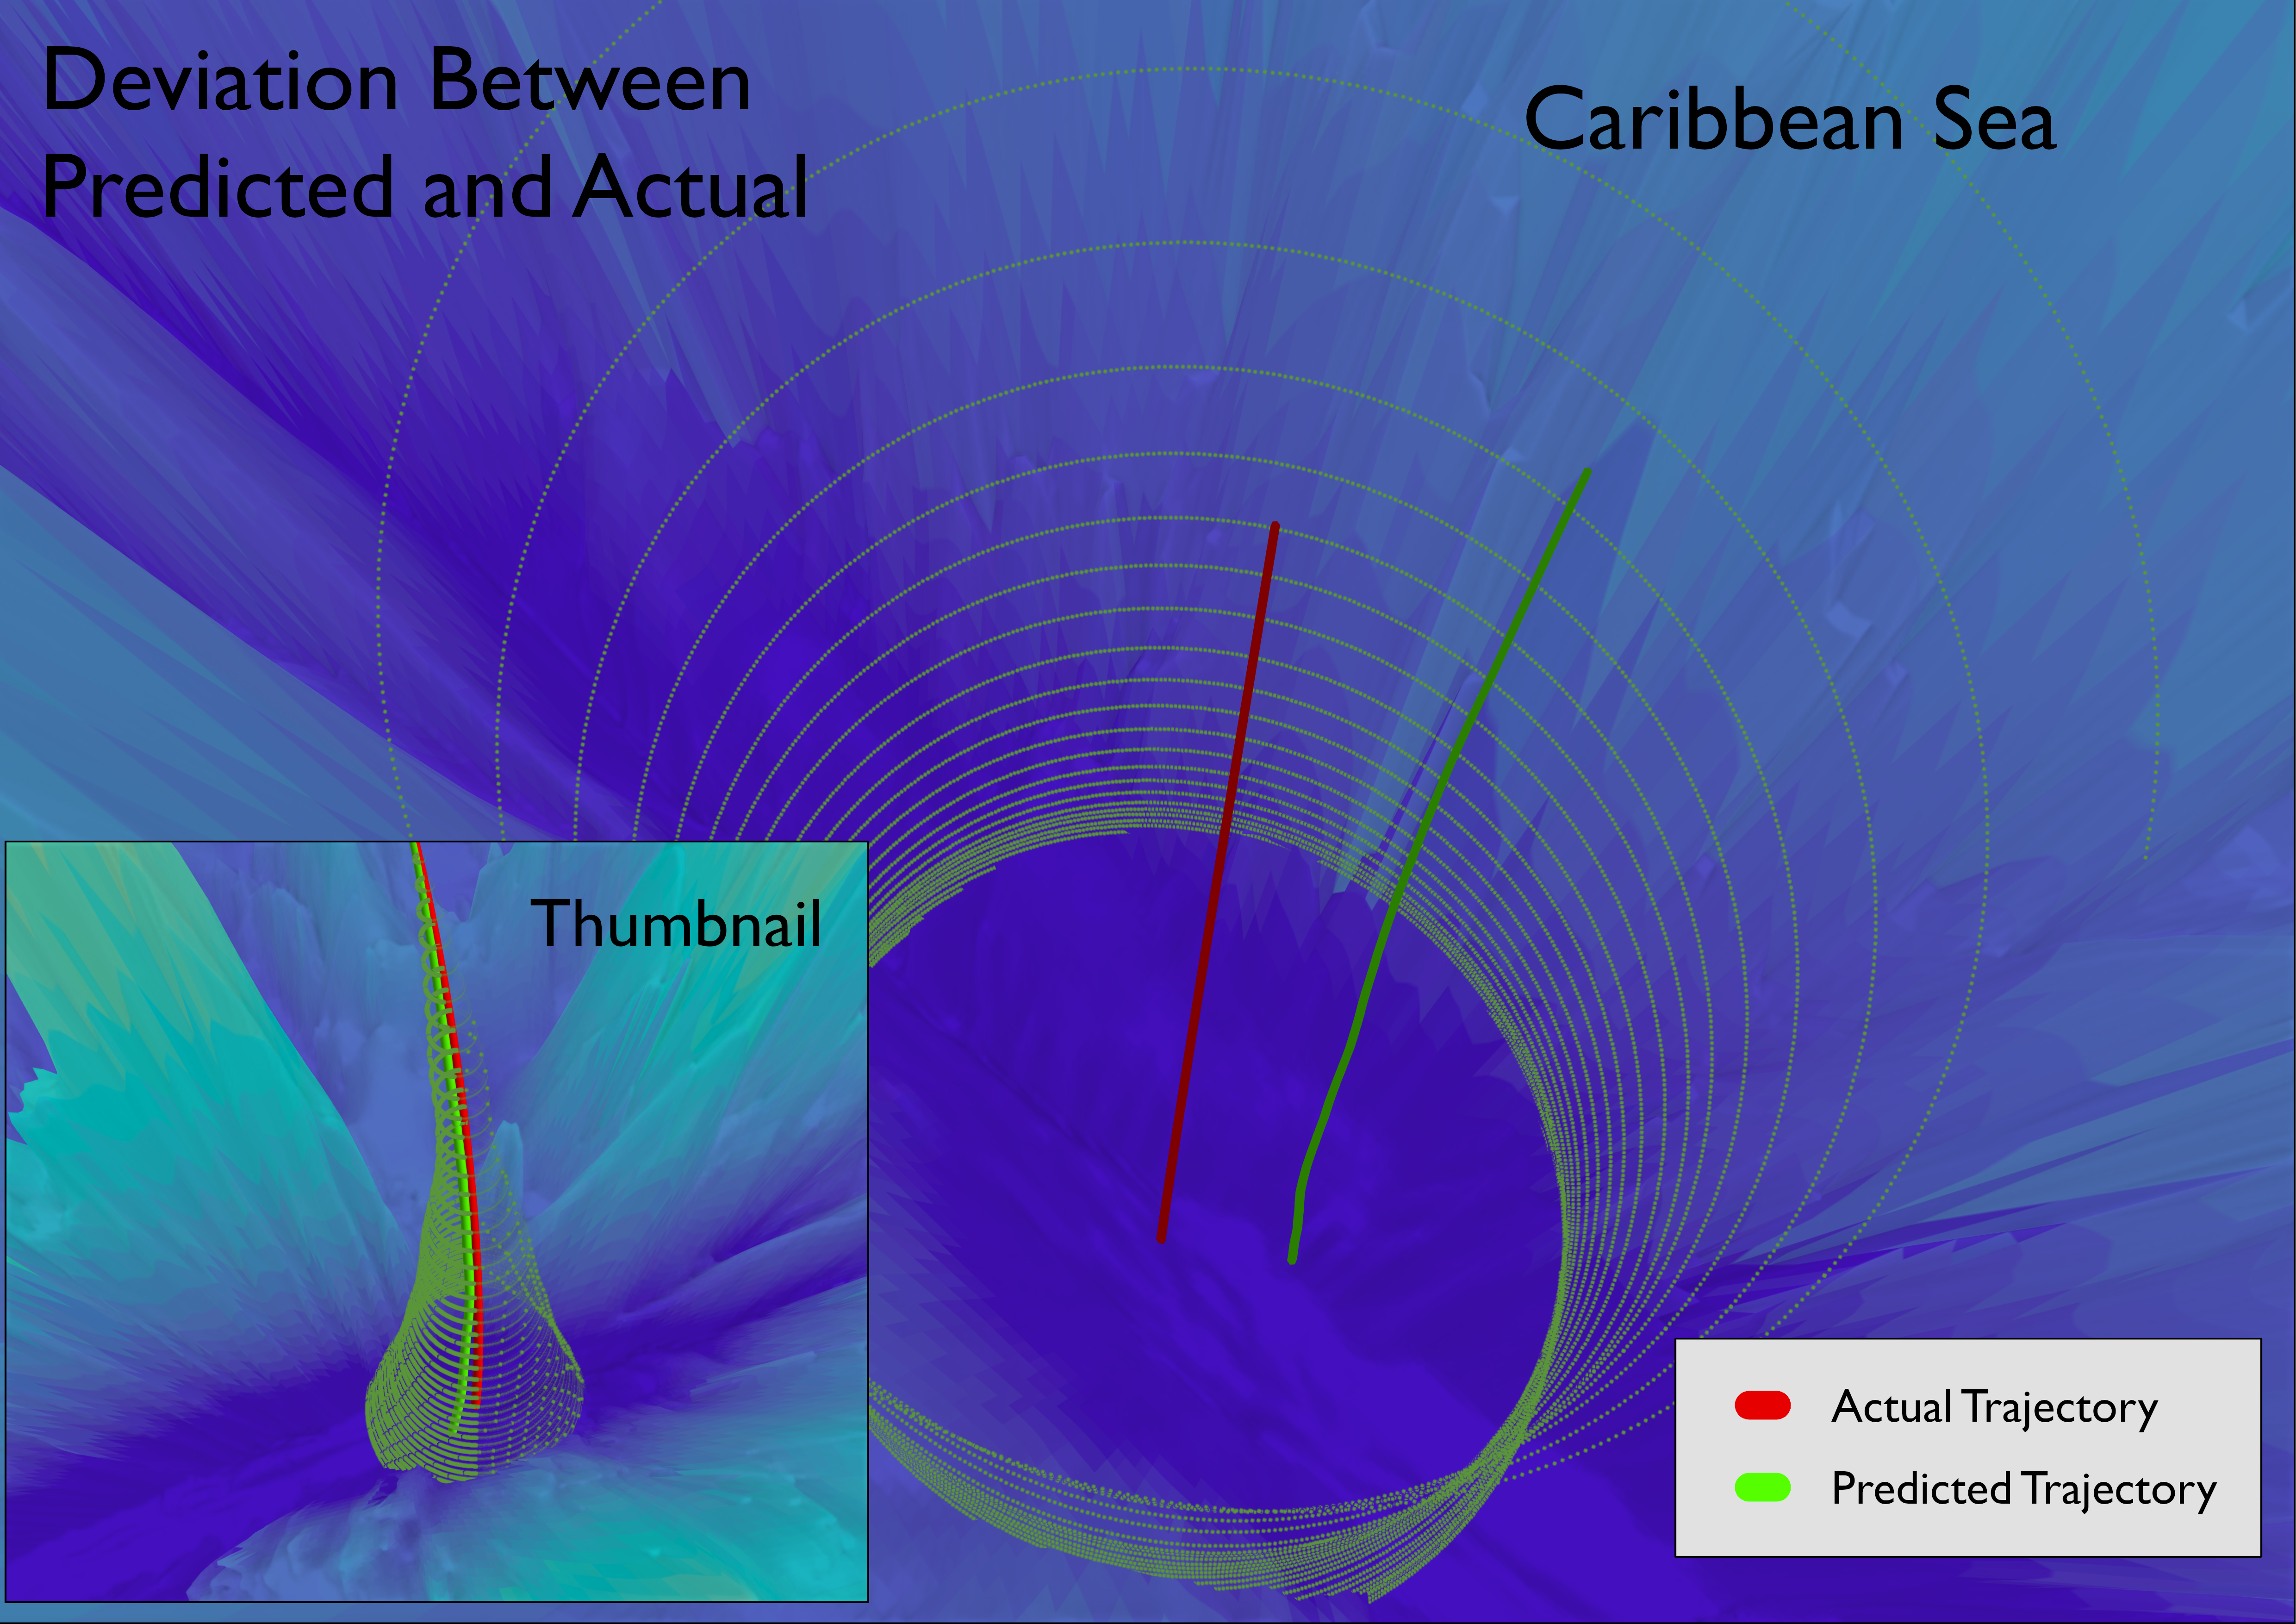
\includegraphics[width=.45\textwidth]{fig/caribbean.jpg} \label{fig:caribbean}
    }
    \subfigure[Model of Multiple Submersibles]{
        \includegraphics[width=.45\textwidth]{fig/multi_submersible.jpg} \label{fig:multi_submersible}
    }
\end{figure}

\section{Model Evaluation and Further Discussion}

\subsection{Pros}

\begin{enumerate}
    \item \textbf{Provides objective evaluation criteria:} Evaluation modeling provides a systematic approach to dealing with complex issues and uses quantitative data for assessment and comparison. This helps to avoid the influence of subjective bias and ensures that evaluation results are objective and credible.
    \item \textbf{Consideration of trade-offs among multiple factors: }Evaluation modeling allows multiple factors to be taken into account and weighed according to their importance and level of impact. This helps to synthesize factors and produce more comprehensive evaluation results.
    \item \textbf{Provide decision support:} Evaluation modeling allows quantitative assessment and comparison of different decision options. This provides strong decision support to decision-makers and helps them make informed decisions.
\end{enumerate}

\subsection{Cons and Improvement}

\begin{enumerate}
    \item \textbf{Over-idealization for uncertain states:} When constructing the model, we did not consider the influence of the deep sea on the positioning instruments, the currents in the vertical direction of the ocean, or the local ecological environment. To solve these problems, we should conduct field surveys, collect relevant local information, and integrate and apply that information in the consideration and analysis of the model, which will greatly promote the development of the model.
    \item \textbf{Data sources are rather scarce:} When building the model, we only focus on the simulation data, neglecting the field survey and the diversity of data sources. To solve this problem, we can learn and use more authoritative software and enrich data sources.
    \item \textbf{Data extraction is limited to one or two regions:} When performing data extraction, we only focused on the Ionian Sea and the Caribbean Sea and failed to notice the uncertainties in other seas, which resulted in our data support being rather thin. To solve this problem, we can look around the world and collect and download as much marine data as possible from all over the world to weaken the specificity of the data.
\end{enumerate}

\addcontentsline{toc}{section}{References}
\bibliographystyle{siam}
\bibliography{bib}

\newpage

% 取消页头
\pagestyle{empty}

\CenterWallPaper{1.1}{fig/mono.jpg}

\begin{center}
    \Huge\textbf{Memorandum}
\end{center}

\textbf{Date:} \today

\textbf{To:} Greek Government Officials

\textbf{From:} COMAP Modeling Team

\textbf{Subject:} The Feasibility of the Model

\hfill

With further exploration of the ocean, submarines have become crucial tools for humans to conduct scientific research, commercial development, and military activities in the deep sea. Equipped with advanced technology and instruments, submarines are capable of carrying out deep-sea exploration, underwater research, oil exploration, underwater archaeology, and rescue missions, among others, contributing to a better understanding of the ocean and providing valuable marine data and information for scientists.

Submarines can conduct long-term observations and data collection in the deep sea. They can penetrate every corner of the ocean to collect precious deep-sea data. However, unlike remotely operated vehicles (ROVs) or autonomous underwater vehicles (AUVs), submarines rely on large surface vessels or platforms for transportation and support. As submarines cannot provide life support for the onboard researchers, a malfunctioning submarine in the 10,000-meter deep sea poses significant risks to the lives and property of those on board.

We are well aware that the safety of submarines has always been a challenging issue. Submarines in the 10,000-meter deep sea require monitoring of their position and status to take timely measures if necessary. This has also become a hot topic of discussion. Solving the safety problems of submarines not only protects the personnel on board but also safeguards the submarines themselves and the important scientific research data they carry.

In this context, our COMAP mathematical modeling team proposed a submarine positioning model based on underwater dynamics to address the monitoring and prediction of submarine positions and statuses in deep-sea environments. To achieve this goal, we utilized advanced underwater dynamics models and timely reports from submarines. Our designed algorithm employs advanced underwater dynamics models to accurately predict the motion trajectory of submarines in deep-sea environments. The reported data from submarines includes parameters measured by sensors, such as depth, speed, and attitude angles, as well as the status information of internal systems, such as remaining battery capacity, operation of motors and servos, and so on. By measuring ocean parameters such as water flow velocity, temperature, and salinity, and analyzing them together with real-time submarine data, we can obtain the position and motion status of submarines in real-time.

At the same time, we also considered the errors caused by environmental factors and incorporated these uncertainties into the algorithm design, analyzing and establishing the corresponding uncertainty evaluation model. By analyzing the reported data and environmental parameters of submarines, we can quantify the magnitude of uncertainties and incorporate them into the prediction model. This way, we can comprehensively evaluate the position and motion status of submarines and provide more accurate prediction results. The uncertainty evaluation model assists us in effectively dealing with errors in submarine positioning and providing accurate position and status information. With this model, we can identify and correct errors caused by environmental factors, thereby improving the accuracy and reliability of position estimation.

While establishing the submarine positioning model, we also took into consideration the issue of rescue equipment selection. To determine the most suitable rescue equipment, we adopted a comprehensive evaluation model based on the Analytic Hierarchy Process (AHP) and the Entropy Weight Method (EWM). In the selection of rescue equipment, we proposed a comprehensive evaluation model based on AHP and EWM to assist us in choosing rescue equipment from both subjective and objective perspectives.

In the event of an accident, our submarine positioning model plays a crucial role. By analyzing the reported data and environmental parameters of the submarine and combining them with our model, we can quickly obtain the position and motion status of the submarine at the time of the incident. This is essential for taking timely and appropriate rescue and response measures. Additionally, the comprehensive evaluation model based on AHP and EWM can provide key information for the selection of rescue equipment.

We also optimized the search path for rescue operations. After a submarine accident, the rescue team needs to quickly and effectively search for and locate the position of the submarine to carry out rescue operations. To optimize the search path, we considered multiple factors. Firstly, we analyzed the motion characteristics and possible positions of the submarine and inferred the probability distribution of possible positions based on the pre-accident trajectory and motion patterns. Then, utilizing our proposed spiral-linear search method, we can increase the probability of finding trapped personnel in the shortest time possible. By planning a reasonable path and employing search strategies, we can assist the rescue team in quickly responding to emergencies, thereby finding and rescuing the submarine in the shortest possible time.

Furthermore, we have also considered the case of multiple submarines. In situations where multiple submarines are present, the positions and motion statuses of each submarine will mutually influence each other. To accurately locate each submarine, we established a model for the interaction between submarines using the principle of momentum and derived equations accordingly. Through the principle of momentum, we can take into account the thrust, drag, and interactions with surrounding water currents experienced by each submarine. Thus, we can derive the motion equations and momentum equations for each submarine, understanding the interactions and influences among them. In situations with multiple submarines, our model comprehensively considers the changes in position, velocity, and forces of each submarine, thereby inferring their motion trajectories and final positions. By modeling the interactions between submarines, we can accurately predict the positions of each submarine and provide real-time updated monitoring and prediction results.

Finally, we conducted tests to evaluate the generalization capability of the model. We conducted tests in the Ionian Sea, an area with complex marine environments and different underwater dynamics characteristics. By conducting actual tests in this sea area, we can verify the performance of the model in real-world conditions and collect actual data for model training and validation. Additionally, to further validate the model's generalization capability, we conducted simulated tests in the Caribbean Sea. The Caribbean Sea has different marine environments and characteristics compared to the Ionian Sea. By conducting tests in this region, we can assess the adaptability of the model to different environments and verify the stability and reliability of its performance.

We believe that the series of models we have established can effectively monitor and ensure the safety of MCMS company's submarines. We sincerely request your support and approval. Through cooperation and collaboration, we will be able to achieve significant results in the monitoring and rescue of submarine safety while contributing to the protection of the marine environment.


\begin{flushright}
    Sincerely,
    
    COMAP Modeling Team
\end{flushright}

\end{document}
\end
